%  LaTeX support: latex@mdpi.com
%  In case you need support, please attach all files that are necessary for compiling as well as the log file, and specify the details of your LaTeX setup (which operating system and LaTeX version / tools you are using).

%=================================================================
\documentclass[psych,tutorial,submit,moreauthors,pdftex]{mdpi}

% If you would like to post an early version of this manuscript as a preprint, you may use preprint as the journal and change 'submit' to 'accept'. The document class line would be, e.g., \documentclass[preprints,article,accept,moreauthors,pdftex]{mdpi}. This is especially recommended for submission to arXiv, where line numbers should be removed before posting. For preprints.org, the editorial staff will make this change immediately prior to posting.

%% Some pieces required from the pandoc template
\providecommand{\tightlist}{%
  \setlength{\itemsep}{0pt}\setlength{\parskip}{4pt}}
\setlist[itemize]{leftmargin=*,labelsep=5.8mm}
\setlist[enumerate]{leftmargin=*,labelsep=4.9mm}

\usepackage{longtable}

% see https://stackoverflow.com/a/47122900
\usepackage{color}
\usepackage{fancyvrb}
\newcommand{\VerbBar}{|}
\newcommand{\VERB}{\Verb[commandchars=\\\{\}]}
\DefineVerbatimEnvironment{Highlighting}{Verbatim}{commandchars=\\\{\}}
% Add ',fontsize=\small' for more characters per line
\usepackage{framed}
\definecolor{shadecolor}{RGB}{248,248,248}
\newenvironment{Shaded}{\begin{snugshade}}{\end{snugshade}}
\newcommand{\AlertTok}[1]{\textcolor[rgb]{0.94,0.16,0.16}{#1}}
\newcommand{\AnnotationTok}[1]{\textcolor[rgb]{0.56,0.35,0.01}{\textbf{\textit{#1}}}}
\newcommand{\AttributeTok}[1]{\textcolor[rgb]{0.77,0.63,0.00}{#1}}
\newcommand{\BaseNTok}[1]{\textcolor[rgb]{0.00,0.00,0.81}{#1}}
\newcommand{\BuiltInTok}[1]{#1}
\newcommand{\CharTok}[1]{\textcolor[rgb]{0.31,0.60,0.02}{#1}}
\newcommand{\CommentTok}[1]{\textcolor[rgb]{0.56,0.35,0.01}{\textit{#1}}}
\newcommand{\CommentVarTok}[1]{\textcolor[rgb]{0.56,0.35,0.01}{\textbf{\textit{#1}}}}
\newcommand{\ConstantTok}[1]{\textcolor[rgb]{0.00,0.00,0.00}{#1}}
\newcommand{\ControlFlowTok}[1]{\textcolor[rgb]{0.13,0.29,0.53}{\textbf{#1}}}
\newcommand{\DataTypeTok}[1]{\textcolor[rgb]{0.13,0.29,0.53}{#1}}
\newcommand{\DecValTok}[1]{\textcolor[rgb]{0.00,0.00,0.81}{#1}}
\newcommand{\DocumentationTok}[1]{\textcolor[rgb]{0.56,0.35,0.01}{\textbf{\textit{#1}}}}
\newcommand{\ErrorTok}[1]{\textcolor[rgb]{0.64,0.00,0.00}{\textbf{#1}}}
\newcommand{\ExtensionTok}[1]{#1}
\newcommand{\FloatTok}[1]{\textcolor[rgb]{0.00,0.00,0.81}{#1}}
\newcommand{\FunctionTok}[1]{\textcolor[rgb]{0.00,0.00,0.00}{#1}}
\newcommand{\ImportTok}[1]{#1}
\newcommand{\InformationTok}[1]{\textcolor[rgb]{0.56,0.35,0.01}{\textbf{\textit{#1}}}}
\newcommand{\KeywordTok}[1]{\textcolor[rgb]{0.13,0.29,0.53}{\textbf{#1}}}
\newcommand{\NormalTok}[1]{#1}
\newcommand{\OperatorTok}[1]{\textcolor[rgb]{0.81,0.36,0.00}{\textbf{#1}}}
\newcommand{\OtherTok}[1]{\textcolor[rgb]{0.56,0.35,0.01}{#1}}
\newcommand{\PreprocessorTok}[1]{\textcolor[rgb]{0.56,0.35,0.01}{\textit{#1}}}
\newcommand{\RegionMarkerTok}[1]{#1}
\newcommand{\SpecialCharTok}[1]{\textcolor[rgb]{0.00,0.00,0.00}{#1}}
\newcommand{\SpecialStringTok}[1]{\textcolor[rgb]{0.31,0.60,0.02}{#1}}
\newcommand{\StringTok}[1]{\textcolor[rgb]{0.31,0.60,0.02}{#1}}
\newcommand{\VariableTok}[1]{\textcolor[rgb]{0.00,0.00,0.00}{#1}}
\newcommand{\VerbatimStringTok}[1]{\textcolor[rgb]{0.31,0.60,0.02}{#1}}
\newcommand{\WarningTok}[1]{\textcolor[rgb]{0.56,0.35,0.01}{\textbf{\textit{#1}}}}

%--------------------
% Class Options:
%--------------------
%----------
% journal
%----------
% Choose between the following MDPI journals:
% acoustics, actuators, addictions, admsci, aerospace, agriculture, agriengineering, agronomy, algorithms, animals, antibiotics, antibodies, antioxidants, applsci, arts, asc, asi, atmosphere, atoms, axioms, batteries, bdcc, behavsci , beverages, bioengineering, biology, biomedicines, biomimetics, biomolecules, biosensors, brainsci , buildings, cancers, carbon , catalysts, cells, ceramics, challenges, chemengineering, chemistry, chemosensors, children, cleantechnol, climate, clockssleep, cmd, coatings, colloids, computation, computers, condensedmatter, cosmetics, cryptography, crystals, dairy, data, dentistry, designs , diagnostics, diseases, diversity, drones, econometrics, economies, education, electrochem, electronics, energies, entropy, environments, epigenomes, est, fermentation, fibers, fire, fishes, fluids, foods, forecasting, forests, fractalfract, futureinternet, futurephys, galaxies, games, gastrointestdisord, gels, genealogy, genes, geohazards, geosciences, geriatrics, hazardousmatters, healthcare, heritage, highthroughput, horticulturae, humanities, hydrology, ijerph, ijfs, ijgi, ijms, ijns, ijtpp, informatics, information, infrastructures, inorganics, insects, instruments, inventions, iot, j, jcdd, jcm, jcp, jcs, jdb, jfb, jfmk, jimaging, jintelligence, jlpea, jmmp, jmse, jnt, jof, joitmc, jpm, jrfm, jsan, land, languages, laws, life, literature, logistics, lubricants, machines, magnetochemistry, make, marinedrugs, materials, mathematics, mca, medicina, medicines, medsci, membranes, metabolites, metals, microarrays, micromachines, microorganisms, minerals, modelling, molbank, molecules, mps, mti, nanomaterials, ncrna, neuroglia, nitrogen, notspecified, nutrients, ohbm, particles, pathogens, pharmaceuticals, pharmaceutics, pharmacy, philosophies, photonics, physics, plants, plasma, polymers, polysaccharides, preprints , proceedings, processes, proteomes, psych, publications, quantumrep, quaternary, qubs, reactions, recycling, religions, remotesensing, reports, resources, risks, robotics, safety, sci, scipharm, sensors, separations, sexes, signals, sinusitis, smartcities, sna, societies, socsci, soilsystems, sports, standards, stats, surfaces, surgeries, sustainability, symmetry, systems, technologies, test, toxics, toxins, tropicalmed, universe, urbansci, vaccines, vehicles, vetsci, vibration, viruses, vision, water, wem, wevj

%---------
% article
%---------
% The default type of manuscript is "article", but can be replaced by:
% abstract, addendum, article, benchmark, book, bookreview, briefreport, casereport, changes, comment, commentary, communication, conceptpaper, conferenceproceedings, correction, conferencereport, expressionofconcern, extendedabstract, meetingreport, creative, datadescriptor, discussion, editorial, essay, erratum, hypothesis, interestingimages, letter, meetingreport, newbookreceived, obituary, opinion, projectreport, reply, retraction, review, perspective, protocol, shortnote, supfile, technicalnote, viewpoint
% supfile = supplementary materials

%----------
% submit
%----------
% The class option "submit" will be changed to "accept" by the Editorial Office when the paper is accepted. This will only make changes to the frontpage (e.g., the logo of the journal will get visible), the headings, and the copyright information. Also, line numbering will be removed. Journal info and pagination for accepted papers will also be assigned by the Editorial Office.

%------------------
% moreauthors
%------------------
% If there is only one author the class option oneauthor should be used. Otherwise use the class option moreauthors.

%---------
% pdftex
%---------
% The option pdftex is for use with pdfLaTeX. If eps figures are used, remove the option pdftex and use LaTeX and dvi2pdf.

%=================================================================
\firstpage{1}
\makeatletter
\setcounter{page}{\@firstpage}
\makeatother
\pubvolume{xx}
\issuenum{1}
\articlenumber{5}
\pubyear{2019}
\copyrightyear{2019}
%\externaleditor{Academic Editor: name}
\history{Received: date; Accepted: date; Published: date}
\updates{yes} % If there is an update available, un-comment this line

%% MDPI internal command: uncomment if new journal that already uses continuous page numbers
%\continuouspages{yes}

%------------------------------------------------------------------
% The following line should be uncommented if the LaTeX file is uploaded to arXiv.org
%\pdfoutput=1

%=================================================================
% Add packages and commands here. The following packages are loaded in our class file: fontenc, calc, indentfirst, fancyhdr, graphicx, lastpage, ifthen, lineno, float, amsmath, setspace, enumitem, mathpazo, booktabs, titlesec, etoolbox, amsthm, hyphenat, natbib, hyperref, footmisc, geometry, caption, url, mdframed, tabto, soul, multirow, microtype, tikz

%=================================================================
%% Please use the following mathematics environments: Theorem, Lemma, Corollary, Proposition, Characterization, Property, Problem, Example, ExamplesandDefinitions, Hypothesis, Remark, Definition
%% For proofs, please use the proof environment (the amsthm package is loaded by the MDPI class).

%=================================================================
% Full title of the paper (Capitalized)
\Title{Reproducible Research in R: A Tutorial on how to Do the Same
Thing More Than Once}

% Authors, for the paper (add full first names)
\Author{Aaron Peikert$^{1, 2,
*}$\href{https://orcid.org/0000-0001-7813-818X}{\orcidicon}, Caspar J.
van Lissa$^{3,
4}$\href{https://orcid.org/0000-0002-0808-5024}{\orcidicon}, Andreas M.
Brandmaier$^{1, 5,
6}$\href{https://orcid.org/0000-0001-8765-6982}{\orcidicon}}

% Authors, for metadata in PDF
\AuthorNames{Aaron Peikert, Caspar J. van Lissa, Andreas M. Brandmaier}

% Affiliations / Addresses (Add [1] after \address if there is only one affiliation.)
\address{%
$^{1}$ \quad Center for Lifespan Psychology---Max Planck Institute for
Human Development, Lentzeallee 94, 14195 Berlin, Germany; \\
$^{2}$ \quad Humboldt-Universität zu Berlin, Berlin, Germany; \\
$^{3}$ \quad Department of Methodology \& Statistics---Utrecht
University, Faculty of Social and Behavioral Sciences, Utrecht,
Netherlands; \\
$^{4}$ \quad Open Science Community Utrecht, Utrecht, Netherlands; \\
$^{5}$ \quad Max Planck UCL Centre for Computational Psychiatry and
Ageing Research Berlin, Germany, and London, UK; \\
$^{6}$ \quad MSB Medical School Berlin, Berlin, Germany; \\
}
% Contact information of the corresponding author
\corres{Correspondence: \href{mailto:peikert@mpib-berlin.mpg.de}{\nolinkurl{peikert@mpib-berlin.mpg.de}}}

% Current address and/or shared authorship








% The commands \thirdnote{} till \eighthnote{} are available for further notes

% Simple summary
\simplesumm{Reproducibility has long been considered integral to the
scientific method. An analysis is considered reproducible if an
independent person can obtain the same results from the same data. Until
recently, detailed descriptions of methods and analyses were the primary
instrument for ensuring scientific reproducibility. Technological
advancements now enable scientists to achieve a more comprehensive
standard that allows anyone to access a digital research repository and
reproduce all computational steps from raw data to final report,
including all relevant statistical analyses, with a single command. This
method has far-reaching implications for scientific archiving,
reproducibility and replication, scientific productivity, and the
credibility and reliability of scientific knowledge. One obstacle to the
widespread use of this method is that the underlying tools are complex
and not part of most researchers' basic training. This paper introduces
\texttt{repro}, an R package that guides researchers through
installation and use of the tools required to make a research project
reproducible. We also suggest using the proposed workflow for the
preregistration of study plans as reproducible computer code
(Preregistration as Code; PAC). Since computer code represents the
planned analyses exactly as they will be executed, it is more precise
than natural language descriptions. PAC circumvents the shortcomings of
ambiguous preregistrations that may result in undisclosed use of
researcher degrees of freedom. Reproducibility, facilitated by
automation, has a wide range of applications and could potentially
accelerate scientific progress.}

% Abstract (Do not insert blank lines, i.e. \\)
\abstract{Computational reproducibility is the ability to obtain
identical results from the \emph{same} data with the \emph{same}
computer code. It is a building block for transparent and cumulative
science because it enables the originator and other researchers, on
other computers and later in time, to reproduce and thus understand how
results came about while avoiding a variety of errors that may lead to
erroneous reporting of statistical and computational results. In this
tutorial, we demonstrate how the R package \texttt{repro} supports
researchers in creating fully computationally reproducible research
projects with tools from the software engineering community. Building
upon this notion of fully automated reproducibility we present several
applications including the preregistration of research plans with code
(Preregistration as Code, PAC). PAC eschews all ambiguity of traditional
preregistration and offers several more advantages. Making technical
advancements that serve reproducibility more widely accessible for
researchers holds the potential to innovate the research process to
become more productive, credible, and reliable.}

% Keywords
\keyword{open science; computational reproducibility; preregistration;
R; R Markdown; Make; GitHub; Docker}

% The fields PACS, MSC, and JEL may be left empty or commented out if not applicable
%\PACS{J0101}
%\MSC{}
%\JEL{}

%%%%%%%%%%%%%%%%%%%%%%%%%%%%%%%%%%%%%%%%%%
% Only for the journal Diversity
%\LSID{\url{http://}}

%%%%%%%%%%%%%%%%%%%%%%%%%%%%%%%%%%%%%%%%%%
% Only for the journal Applied Sciences:
%\featuredapplication{Authors are encouraged to provide a concise description of the specific application or a potential application of the work. This section is not mandatory.}
%%%%%%%%%%%%%%%%%%%%%%%%%%%%%%%%%%%%%%%%%%

%%%%%%%%%%%%%%%%%%%%%%%%%%%%%%%%%%%%%%%%%%
% Only for the journal Data:
%\dataset{DOI number or link to the deposited data set in cases where the data set is published or set to be published separately. If the data set is submitted and will be published as a supplement to this paper in the journal Data, this field will be filled by the editors of the journal. In this case, please make sure to submit the data set as a supplement when entering your manuscript into our manuscript editorial system.}

%\datasetlicense{license under which the data set is made available (CC0, CC-BY, CC-BY-SA, CC-BY-NC, etc.)}

%%%%%%%%%%%%%%%%%%%%%%%%%%%%%%%%%%%%%%%%%%
% Only for the journal Toxins
%\keycontribution{The breakthroughs or highlights of the manuscript. Authors can write one or two sentences to describe the most important part of the paper.}

%\setcounter{secnumdepth}{4}
%%%%%%%%%%%%%%%%%%%%%%%%%%%%%%%%%%%%%%%%%%

% Pandoc citation processing

\DefineVerbatimEnvironment{Highlighting}{Verbatim}{commandchars=\\\{\}, numbers=left}

\begin{document}
%%%%%%%%%%%%%%%%%%%%%%%%%%%%%%%%%%%%%%%%%%

\captionsetup{labelformat=empty}

\hypertarget{introduction}{%
\section{Introduction}\label{introduction}}

Scientists increasingly strive to make research data, materials, and
analysis code openly available. Sharing these digital research products
can increase scientific efficiency by enabling researchers to learn from
each other, reuse materials, and increase scientific reliability by
facilitating the review and replication of published research results.
To some extent, these potential benefits are contingent on whether these
digital research products are reproducible. Reproducibility can be
defined as the ability of anyone to obtain identical results from the
\emph{same} data with the \emph{same} computer code \citep[see][ for
details]{Peikert2019}. The credibility of empirical research results
hinges on their objectivity. Objectivity in this context means, ``in
principle it {[}the research finding{]} can be tested and understood by
anybody.'' \citep[p.~22]{popperLogicScientificDiscovery2002}. Only a
reproducible result meets these requirements. Therefore, reproducibility
has long been considered integral to empirical research. Unfortunately,
despite increasing commitment to open science practices and good will,
many projects can not yet be reproduced by other research teams
\citep{obels2020}. This is because there are various challenges to
making a research project reproducible (e.g., missing software
dependencies or ambiguous documentation of the exact computational steps
taken), and there is a lack of best practices for overcoming these
challenges \citep[but see][]{vanlissa2020worcs}. With technological
advancement, however, it is now possible to make all digital products
related to a research project available in a manner that enables
automatic reproduction of the research project with minimal effort.

With this paper, we pursue two aims. First, we want to introduce
researchers to a notion of automated reproducibility that requires no
manual steps, apart from the initial setup of the software environment.
Secondly, we discuss the implications of automated reproducibility for
changing the general approach to research. With regard to the first
goal, we discuss how to address four common threats to reproducibility,
using tools originating from software engineering \citep[see][ for
details]{Peikert2019}, and present a tutorial on how to employ these
tools to achieve automated reproducibility. A single tutorial cannot
comprehensively introduce the reader to the detail of individual tools,
but this tutorial is intended to help readers get started with a basic
workflow. The tutorial is aimed at researchers who regularly write code
to analyze their data and are willing to make relevant code, data, and
materials available, either publicly or on request. Ideally, the reader
has already created a dynamic document at some point in time (e.g., with
R Markdown or Jupyter) and used some form of version control (e.g.,
Git). The R package \texttt{repro} supports researchers in setting up
the required software and in adopting this workflow. We present
automated reproducibility as a best practice; a goal that is not always
fully achieved due to limited resources, technical restrictions, or
practical considerations, but is worth striving for nonetheless.

In pursuit of the second aim, we present a strictly reproducible and
unambiguous form of preregistration \citep{NosekRevolution2018} that
builds upon implementing this reproducible workflow, the so-called
\emph{Preregistration as Code} (PAC). PAC involves preregistering the
intended analysis code and the major part of the final scientific report
as a dynamic document, including typical sections like introduction,
methods, and results. The resulting dynamic document closely resembles
the final manuscript but uses simulated data to generate placeholder
results (e.g., figures, tables, and statistics). Simulated data serve
two functions, they allow to test the code for the planned analyses and
for preregistering the exact presentation of the results. Once the
empirical data are available, these replace the simulated data; the
results are then updated automatically, and the discussion can be
written to finalize the report.

Scientific organizations and funding bodies increasingly demand
transparent sharing of digital research products, and researchers are
increasingly willing to do so. However, although the sharing of such
digital research products is a necessary condition for reproducibility,
it is not a sufficient one. This was illustrated by an attempt to
reproduce results from open materials in the journal \emph{Cognition}
\citep{hardwicke2018}. Out of 35 published articles with open code and
data, results of 22 articles could be reproduced, but in 11 of these
cases, further assistance from the original authors was required. For 13
articles, at least 1 outcome could not be reproduced-----even with the
original authors' assistance. Another study of 62 Registered Reports
found that only 41 had data available, and 37 had analysis scripts
available \citep{obels2020}. The authors could execute only 31 of the
scripts without error and reproduce the results of only 21 articles
(within a reasonable time). These failed attempts to reproduce findings
highlight the need for widely accepted reproducibility standards because
open repositories do not routinely provide sufficient information to
reproduce relevant computational and statistical results. If digital
research products are available but not reproducible, their added value
is limited.

This tutorial demonstrates how R users can make digital research
products more reproducible, while striking a balance between rigor and
ease-of-use. A rigorous standard increases the likelihood that a project
will remain reproducible as long as possible. An easy-to-use standard,
on the other hand, is more likely to be adopted. Our approach is to
promote broad adoption of such practices by ensuring a ``low
threshold'', by making it easy to get started, while enabling a ``high
ceiling'' by ensuring that they are compatible with more complex
rigorous solutions. As researchers become more proficient in using the
tools involved, they can thus further improve the reproducibility of
their work.

We have structured the tutorial with a \emph{learning-by-doing} approach
in mind, such that readers can follow along on their own computers. We
explicitly encourage readers to try out all R commands for themselves.
Unless stated otherwise, all code blocks are meant to be run in the
statistical programming language R \citep[tested with version
4.0.4]{R-base}.

\hypertarget{threats-to-reproducibility-and-appropriate-remedies}{%
\section{Threats to Reproducibility and Appropriate
Remedies}\label{threats-to-reproducibility-and-appropriate-remedies}}

From our own experience with various research projects, we have
identified the following common threats to reproducibility:

\begin{enumerate}
\def\labelenumi{\arabic{enumi}.}
\tightlist
\item
  \emph{Multiple inconsistent versions of code, data, or both}; for
  example, the data set may have changed over time because outliers were
  removed at a later stage or an item was later recoded; or, the
  analysis code may have been modified during the writing of a paper
  because a bug was removed at some point in time. It may then be
  unclear which version of code and data was used to produce some
  reported set of results.
\item
  \emph{Copy-and-paste errors}; for example, results are often manually
  copied from a statistical computing language into a text processor; if
  a given analysis is re-run and results are manually updated in the
  text processor, this may inadvertently lead to inconsistencies between
  the reported result and the reproduced result.
\item
  \emph{Undocumented or ambiguous order of computation}; for example,
  with multiple data and code files, it may be unclear which scripts
  should be executed in what order; or, some of the computational steps
  are documented (e.g., final analysis), but other steps were conducted
  manually without documentation (e.g., executing a command manually
  rather than in a script; copy-and-pasting results from one program to
  another).
\item
  \emph{Ambiguous software dependencies}; for example, a given analysis
  may depend on a specific version of a specific software package, or
  rely on software that might not be available on a different computer,
  or no longer exist at all; or a different version of the same software
  may produce different results.
\end{enumerate}

We have developed a workflow that achieves long-term and cross-platform
computational reproducibility of scientific data analyses. It leverages
established tools and practices from software engineering and rests on
four pillars that address the aforementioned causes of
non-reproducibility \citep{Peikert2019}:

\begin{enumerate}
\def\labelenumi{\arabic{enumi}.}
\tightlist
\item
  Version control
\item
  Dynamic document generation
\item
  Dependency tracking
\item
  Software management
\end{enumerate}

The remainder of this section briefly explains why each of these four
building blocks is needed and details their role in ensuring
reproducibility. A more extensive treatment of these tools is given in
\citet{Peikert2019}.

\emph{Version control} prevents the ambiguity that arises when multiple
versions of code and data are created in parallel during the lifetime of
a research project. Version control allows a clear link between which
results were generated by which version of code and data. This addresses
the first threat to reproducibility, because results can only be said to
be reproducible if it is clear which version of data and code produced
them. We recommend using \texttt{Git} for version control, because of
its widespread adoption in the R community.

\texttt{Git} tracks changes to all project-related files (e.g.,
materials, data, and code) over time. At any stage, individual files or
the entire project can be compared to, or reverted to, an earlier
version. Moreover, contributions (e.g., from collaborators) can be
compared to, and incorporated in the main version of the project.
Version control thus reduces the risk of losing work and facilitates
collaboration. \texttt{Git} is built around snapshots that represent the
project state at a given point in time. These snapshots are called
\emph{commits} and work like a ``save'' action. Ideally, each commit has
a message that succinctly describes these changes. It is good practice
to make commits for concrete milestones (e.g., ``Commented on
Introduction,'' ``Added SES as a covariate,'' ``Address Reviewer 2's
comment 3''). This makes it easier to revert specific changes than when
multiple milestones are joined in one commit, e.g., ``Changes made on
19/07/2021''. Each commit refers back to its ancestor, and all commits
are thus linked in a timeline. The entirety of commits (i.e., the
version-controlled project) is called a repository. In \texttt{Git},
specific snapshots of a repository can be tagged, such that the user can
clearly label which version of the project was used to create a
preregistration, preprint, or final version of the manuscript as
accepted by a journal. \texttt{Git} has additional features beyond basic
version control, such as ``branches'' (parallel versions of a project
that can later be merged again) to facilitate simultaneous
collaboration. \citet{vuorreCuratingResearchAssets2018} provide a more
extensive treatment of how \texttt{Git} functions and how to use
\texttt{Git} for research. \citet{bryanExcuseMeYou2018} provides
additional information on how to track \texttt{R\ Markdown} documents.
Collaborating via \texttt{Git} is facilitated by uploading the
repository to a cloud-based service. We recommend GitHub as a host for
\texttt{Git} repositories because of its popularity among R users.
GitHub has many tools that facilitate working with \texttt{Git} --- in
particular project management and collaboration --- but these are not
central to achieving reproducibility.

Second, we rely on \emph{dynamic document generation}. The traditional
way of writing a scientific report based on a statistical data analysis
uses two separate steps conducted in two different programs. The
researcher writes text in a word processor, and conducts the analysis in
another program. Results are then (manually) copied and pasted from one
program to another, a process that often produces inconsistencies
\citep{nuijtenPrevalenceStatisticalReporting2016}.

Dynamic document generation integrates both steps. Through dynamic
document generation, code becomes an integral, although usually hidden,
part of the manuscript, complementing the verbal description and
allowing interested readers to gain a deeper understanding of the
contents
\citep{knuthCWEBSystemStructured, claerboutElectronicDocumentsGive1992}.
\texttt{R\ Markdown} uses \texttt{Markdown} for text formatting and R
(or other programming languages) for writing the statistical analysis.
\texttt{Markdown} is a lightweight text format in plain text with a
minimal set of reserved symbols for formatting instructions. This way,
\texttt{Markdown} does not need any specialized software for editing. It
is userfriendly (unlike, for example, \texttt{LaTeX}
\citep{lamportLATEXDocumentPreparation1994}), works well with version
control systems, and can be exported to various document formats, such
as HTML websites, a Microsoft Word document, a typeset PDF file (for
example, via LaTeX journal templates), or a Powerpoint presentation.
\texttt{Markdown} can be used for all sorts of academic documents,
ranging from simple sketches of ideas to scientific manuscripts
\citep{R-rticles} and presentations \citep{revealjs}, or even résumés
\citep{vitae}. \texttt{R\ Markdown} extends regular \texttt{Markdown} by
allowing users to include R code chunks (in fact, arbitrary computer
code \citep[Chapter 15, Chapter 15, Other
Languages]{xieMarkdownCookbook2020}) into a \texttt{Markdown} document.
Upon rendering the document, the code blocks are executed, and their
output is dynamically inserted into the document. This allows the
creation of (conditionally) formatted text, statistical results, and
figures that are guaranteed to be up-to-date because they are created
anew every time the document is rendered to its output format (e.g.,
presentation slides or a journal article).
\citet{xieMarkdownCookbook2020} provides an extensive yet practical
introduction to most features of \texttt{R\ Markdown}.

While version control and dynamic document generation are becoming more
common, we have argued that two more components are required and that
each component alone is unlikely to guarantee reproducibility
\citep{Peikert2019, vanlissa2020worcs}. In practice, dependencies
between project files (e.g., information on what script uses which data
file and what script needs to be run first) or on external software
(e.g., system libraries or components of the programming language, such
as other R packages) are frequently unmentioned or not exhaustively and
unambiguously documented.

\emph{Dependency tracking} helps automatically resolve dependencies
between project files. In essence, researchers provide a collection of
\emph{computational recipes}. A computational recipe describes how
inputs are processed to deterministically create a specific output in a
way that is automatically executable. The concept of computational
recipes is central to our understanding of reproducibility because it
enables a unified way to reproduce a project automatically. Similar to a
collection of cooking recipes, we can have multiple products
(\emph{targets}) with different ingredients (\emph{requirements}) and
different steps of preparation (\emph{recipes}). In the context of
scientific data analysis, targets are typically the final scientific
report (e.g., the one to be submitted to a journal) and possibly
intermediate results (such as preprocessed data files, simulation
results, and analysis results). A workflow that involves renaming
variable names by hand in a graphical spreadsheet application, for
example, is therefore incompatible with automated reproducibility.
Another property of a computational recipe is that the same inputs
should always result in the same outputs. For most computer code (given
the same software is used), this property is fulfilled. However, one
noteworthy exception is the generation of pseudo-random numbers.
Whenever random numbers are used in a computation, it is only
reproducible if the random number generator generates the same numbers.
To ensure identical random numbers, users may fix the state of the
random number generated with a so-called seed (e.g.~\texttt{set.seed()}
in R), but they also need to guarantee that the pseudo-random number
generator is unchanged \citep[see][]{Peikert2019}.

We recommend using \texttt{Make} for dependency tracking because it is
language independent. The following hypothetical example illustrates the
utility of \texttt{Make} and a suitable \texttt{Makefile}. Consider a
research project that contains a script to simulate data
(\texttt{simulate.R}) and a scientific report of the simulation results
written in \texttt{R\ Markdown} (\texttt{manuscript.Rmd}). A
\texttt{Makefile} for this project could look like this:

\begin{Shaded}
\begin{Highlighting}[]
\ExtensionTok{manuscript.pdf:}\NormalTok{ manuscript.Rmd simulated\_data.csv}
  \ExtensionTok{Rscript} \AttributeTok{{-}e} \StringTok{\textquotesingle{}rmarkdown::render("manuscript.Rmd")\textquotesingle{}}

\ExtensionTok{simulated\_data.csv:}\NormalTok{ simulate.R}
  \ExtensionTok{Rscript} \AttributeTok{{-}e} \StringTok{\textquotesingle{}source("simulate.R")\textquotesingle{}}
\end{Highlighting}
\end{Shaded}

There are two targets, the final rendered report
(\texttt{manuscript.pdf}, l. 1) and the simulation results
(\texttt{simulation\_results.csv}, l. 4). Each target is followed by a
colon and a list of requirements. If a requirement is newer than the
target, the recipe will be executed to rebuild the target. If a
requirement does not exist, \texttt{Make} uses a recipe to build the
requirement before building the target. Here, if one were to build the
final \texttt{manuscript.pdf} by rendering the \texttt{R\ Markdown} with
the command shown in l.2, \texttt{Make} would check whether the file
\texttt{simulation\_results.csv} exists; if not, it would issue the
command in l.5 to run the simulation before rendering the manuscript.
This ensures that the simulated data are present before the manuscript
is built, and that the simulation is re-run and the manuscript is
rebuilt if the simulation code was changed. \texttt{Make} therefore
offers a standardized process to reproduce projects, regardless of the
complexity or configuration of the project. Note that the Workflow for
Open Reproducible Code in Science (WORCS) we presented elsewhere
\citep{vanlissa2020worcs} does not explicitly contain this dependency
tracking element, but its strict structure of only containing one
definite \texttt{R\ Markdown} still makes dependencies between files
unambiguous.

A version-controlled dynamic document with dependency tracking still
relies on external software. Troubleshooting issues specific to a
particular programming language or dependent tool typically require
considerable expertise and threaten reproducibility. \emph{Software
management} refers to the act of providing records of, or access to, all
software packages and system libraries a project depends on. One
comprehensive approach to software management is containerization. The
central idea is that by ``{[}..{]} packaging the key elements of the
computational environment needed to run the desired software {[}makes{]}
the software much easier to use, and the results easier to reproduce
{[}\ldots{]}'' \citep[p.~174]{silverSoftwareSimplified2017}.

\emph{\texttt{Docker}} is a popular tool for containerization. It
manages software dependencies by constructing a virtual software
environment independent of the host software environment. These
so-called ``\texttt{Docker} images'' function like a virtual computer
(i.e., a ``sand box'' a computational environment seperated from the
host). A \texttt{Docker} image contains \emph{all} software dependencies
used in an analysis---not just R packages, but also R and Rstudio, and
even the operating system. This is important because low level
functionality may impact the workings of higher-order software like R,
such as calls to random number generators or linear algebra libraries.
All of the differences in computational results that could be caused by
variation in the software used are hence eliminated.

Note that the software environment of the Docker image is completely
separate from the software installed on your computer. This separation
is excellent for reproducibility but takes some getting used to. For
example, it is important to realize that software available on your
local computer will \emph{not} be accessible within the confines of the
\texttt{Docker} image. Each dependency that you want to use within the
\texttt{Docker} image must be explicitly added as a dependency.
Furthermore, using \texttt{Docker} may require you to install software
on an operating system that may not be familiar to you. The images
supplied by the rocker project
\citep{boettigerIntroductionRockerDocker2017}, for example, are based on
Linux.

There are two ways to build a \texttt{Docker} image. First, users can
manually install whatever software they like from within the virtual
environment. Such a manually build environment can still be ported to
all computers that support \texttt{Docker}. However, we prefer the
second way of building images automatically from a textual description
called \texttt{Dockerfile}. Because the \texttt{Dockerfile} clearly
describes how which software is installed, the installation process can
be repeated automatically. Users can therefore quickly change the
software environment, for example, update to another R version or given
package version. Packaging all required software in such an image
requires considerable amounts of storage space. Two major strategies
help to keep the storage requirements reasonable. One is to rely on
pre-made images that are maintained by a community for particular
purposes. For example, there are pre-made images that only include what
is necessary for R, based on Ubuntu containers
\citep{boettigerIntroductionRockerDocker2017}. Users can then install
whatever they need in addition to what is provided by these pre-compiled
images. The image that was used for this article uses 1.35GiB of disk
space. The image for this project includes Ubuntu, R, RStudio, LaTeX as
well as a variety of R packages like tidyverse \citep{tidyverse} and all
its dependent packages, amounting to 192 R packages.

A second strategy is to save a so-called \texttt{Dockerfile}, which
contains only a textual description of all commands that need to be
executed to recreate the software environment. \texttt{Dockerfiles} are
tiny (the
\href{https://github.com/aaronpeikert/repro-tutorial/blob/main/Dockerfile}{\texttt{Dockerfile}}
for this project has a size of only 1.55KiB). However, they rely on the
assumption that all software repositories that provide the dependent
operating systems, pieces of software, and R packages will continue to
remain accessible and provide historic software versions. For proper
archiving, we therefore recommend storing a complete image of the
software environment, in addition to the \texttt{Dockerfile}. A more
comprehensive overview of the use of containerization in research
projects is given by
\citet{wiebelsLeveragingContainersReproducible2021}. Note that WORCS,
which we presented elsewhere \citep{vanlissa2020worcs} relies on the R
package \texttt{renv} \citep{R-renv} for software management.
\texttt{renv} is more lightweight and easier to use than \texttt{Docker}
on the one hand, but not as comprehensive on the other because it only
takes snapshots of the R packages instead of all software used.

To summarize, the workflow by \citet{Peikert2019} requires four
components (see Figure 2.1) dynamic document generation (using
\texttt{R\ Markdown}), version control (using \texttt{Git}), dependency
tracking (using \texttt{Make}), and software management (using
\texttt{Docker}). While \texttt{R\ Markdown} and \texttt{Git} are well
integrated into the R environment through RStudio, \texttt{Make} and
\texttt{Docker} require a level of expertise that is often beyond the
training of scholars outside the field of information technology. This
presents a considerable obstacle to the acceptance and implementation of
the workflow. To overcome this obstacle, we have developed the R package
\texttt{repro} that supports scholars in setting up, maintaining, and
reproducing research projects in R. Importantly, a reproducible research
project created with \texttt{repro} does not have the \texttt{repro}
package itself as a dependency. These projects will remain reproducible
irrespective of whether \texttt{repro} remains accessible in future.
Users do not need to have \texttt{repro} installed to reproduce a
project; in fact, they do not even need to have R installed because the
entire project can be rebuilt inside a container with R installed. In
the remainder, we will walk you through the creation of a reproducible
research project with the package \texttt{repro}.

\begin{figure}
\centering
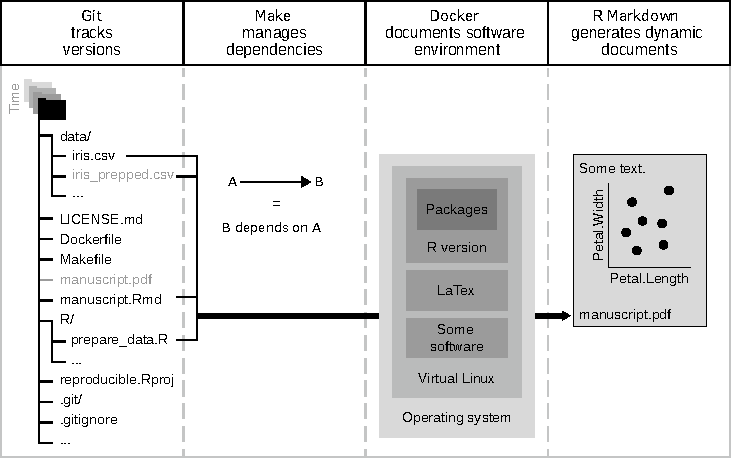
\includegraphics{/home/rstudio/images/nutshell.pdf}
\caption{Figure 2.1: Schematic illustration of the interplay of the four
components (in dashed columns) central to the reproducible workflow:
version control (\texttt{Git}), dependency tracking (\texttt{Make}),
software management (\texttt{Docker}), and dynamic document generation
(\texttt{R\ Markdown}). \texttt{Git} tracks changes to the project over
time. \texttt{Make} manages dependencies among the files.
\texttt{Docker} provides a container in which the final report is built
using dynamic document generation in \texttt{R\ Markdown}. Adapted from
\citet{Peikert2019} licensed under
\href{https://creativecommons.org/licenses/by/4.0}{CC BY 4.0}.}
\end{figure}

\hypertarget{creating-reproducible-research-projects}{%
\section{Creating Reproducible Research
Projects}\label{creating-reproducible-research-projects}}

One impediment to the widespread adoption of a standard for reproducible
research is that learning to use the required tools can be quite
time-intensive. To lower the threshold, the R package \texttt{repro}
introduces helper functions that simplify the use of complicated and
powerful tools. The \texttt{repro} package follows the format of the
\href{https://usethis.r-lib.org}{\texttt{usethis}} \citep{usethis}
package, which provides helper functions to simplify the development of
R packages. The \texttt{repro} package provides similar helper
functions, but focuses on reproducibility-specific utilities. These
helper functions guide end-users in the use of reproducibility tools,
provide feedback about what the computer is doing and suggest what the
user should do next. We hope this makes reproducibility tools more
accessible by enabling beginner-level users to detect their system's
state accurately and act correspondingly \citep[Chapter 8: ``Automation
and Situation Awareness'']{parasuramanAutomationHumanPerformance2018}.
These wrappers are merely a support system; as users learn to use the
underlying tools, they can rely less on \texttt{repro} and use these
tools directly to solve more complex problems.

This tutorial assumes that the user will be working predominantly in R,
with the help of RStudio. It describes basic steps that we expect to be
relevant for small-scale psychological research projects that do not
rely on external software or multistage data processing (for those
requirements see section \protect\hyperlink{advanced-features}{Advanced
Features}). Of course, your specific situation might involve additional,
more specialized steps. After completing the tutorial, you should be
able to customize your workflow accordingly.

The first step is to install the required software. We assume that you
have installed R \citep[version 4.0.4]{R-base} and RStudio
\citep[version 1.4]{rstudio} already but the tutorial will guide you in
detail through the installation of other necessary software with the
help of the R package
\href{https://github.com/aaronpeikert/repro}{\texttt{repro}}
\citep{R-repro}. In case you have either not installed R and RStudio or
are unsure if they are up-to-date, you might want to consult our
installation advice in the
\href{https://github.com/aaronpeikert/repro-tutorial/blob/main/install.md}{Online
Supplementary Material} that covers the installation of all software
necessary for this tutorial in three steps. The
\href{(https://github.com/aaronpeikert/repro-tutorial/blob/main/install.md)}{installation
advice} may also help Windows users who have problems installing
\texttt{Docker}.

Unfortunately, Docker requires administrator rights to run, which may
not be available to all researchers. We recommend
\href{https://rstudio.github.io/renv/articles/renv.html}{\texttt{renv}}
\citep{R-renv} in cases where no administrator rights can be obtained
but can not detail its use in this document. \texttt{renv} tracks which
R package is installed from which source in which version in a so-called
\href{https://rstudio.github.io/renv/articles/lockfile.html}{\texttt{lockfile}}.
This lockfile is then used to reinstall the same packages on other
computers or later in time. For a more thorough discussion, see
\citet{vanlissa2020worcs}.

Start RStudio and install the package
\href{https://github.com/aaronpeikert}{\texttt{repro}}\citep{R-repro}.
It will assist you while you follow the tutorial.

\begin{Shaded}
\begin{Highlighting}[]
\CommentTok{\# repro is not on CRAN yet}
\FunctionTok{options}\NormalTok{(}
  \AttributeTok{repos =} \FunctionTok{c}\NormalTok{(}\AttributeTok{aaronpeikert =} \StringTok{\textquotesingle{}https://aaronpeikert.r{-}universe.dev\textquotesingle{}}\NormalTok{,}
            \AttributeTok{CRAN =} \StringTok{\textquotesingle{}https://cloud.r{-}project.org\textquotesingle{}}\NormalTok{)}
\NormalTok{)}
\FunctionTok{install.packages}\NormalTok{(}\StringTok{\textquotesingle{}repro\textquotesingle{}}\NormalTok{)}
\end{Highlighting}
\end{Shaded}

To verify that you have indeed installed and set up the required
software for this workflow, you can use the ``check functions''. These
also illlustrate how \texttt{repro} assists the user in setting up a
reproducible workflow. In the example below, we use the double-colon
operator to explicitly indicate which functions originate in the
\texttt{repro} package. If the package is loaded (using
\texttt{library("repro")}), it is not necessary to use this double-colon
notation.

\begin{Shaded}
\begin{Highlighting}[]
\CommentTok{\# \textasciigrave{}package::function()\textasciigrave{} → use function from package without \textasciigrave{}library(package)\textasciigrave{}}
\NormalTok{repro}\SpecialCharTok{::}\FunctionTok{check\_git}\NormalTok{()}
\end{Highlighting}
\end{Shaded}

\begin{verbatim}
## v Git is installed, don't worry.
\end{verbatim}

\begin{Shaded}
\begin{Highlighting}[]
\NormalTok{repro}\SpecialCharTok{::}\FunctionTok{check\_make}\NormalTok{()}
\end{Highlighting}
\end{Shaded}

\begin{verbatim}
## v Make is installed, don't worry.
\end{verbatim}

\begin{Shaded}
\begin{Highlighting}[]
\NormalTok{repro}\SpecialCharTok{::}\FunctionTok{check\_docker}\NormalTok{()}
\end{Highlighting}
\end{Shaded}

\begin{verbatim}
## v Docker is installed, don't worry.
\end{verbatim}

These functions check whether specific dependencies are available on the
user's system, and if not, explain what further action is needed to
obtain it. Sometimes they ask the user to take action; for example, the
following happens if you are a Windows user who does not have
\texttt{Git} installed:

\begin{Shaded}
\begin{Highlighting}[]
\NormalTok{repro}\SpecialCharTok{::}\FunctionTok{check\_git}\NormalTok{()}
\end{Highlighting}
\end{Shaded}

\begin{verbatim}
## x Git is not installed.
\end{verbatim}

\begin{verbatim}
## i We recommend Chocolately for Windows users.
\end{verbatim}

\begin{verbatim}
## x Chocolately is not installed.
\end{verbatim}

\begin{verbatim}
## * To install it, follow directions on: 
##   'https://chocolatey.org/docs/installation'
\end{verbatim}

\begin{verbatim}
## i Use an administrator terminal to install chocolately.
\end{verbatim}

\begin{verbatim}
## * Restart your computer.
\end{verbatim}

\begin{verbatim}
## * Run `choco install -y git` in an admin terminal to install Git.
\end{verbatim}

The messages from \texttt{repro} try to help the user solve problems.
They are adjusted to your specific operating system and installed
dependencies. Before you continue, we ask you to run the above commands
to check \texttt{Git}, \texttt{Make}, and \texttt{Docker}---both to
become familiar with the functionality of the \texttt{check\_*()}
functions and to make sure your system is prepared for the remainder of
this tutorial.

After you have installed the necessary software, we suggest that you set
up a secure connection to GitHub:

\begin{Shaded}
\begin{Highlighting}[]
\NormalTok{repro}\SpecialCharTok{::}\FunctionTok{check\_github}\NormalTok{()}
\end{Highlighting}
\end{Shaded}

\begin{verbatim}
## v You and GitHub are on good terms, don't worry.
\end{verbatim}

If you know what Secure Shell (SSH) is and want to use it, you may
alternatively use:

\begin{Shaded}
\begin{Highlighting}[]
\CommentTok{\# only an alternative: DO NOT USE if you are unsure what SSH means}
\NormalTok{repro}\SpecialCharTok{::}\FunctionTok{check\_github}\NormalTok{(}\AttributeTok{auth\_method =} \StringTok{"ssh"}\NormalTok{)}
\end{Highlighting}
\end{Shaded}

\begin{verbatim}
## v You and GitHub are on good terms, don't worry.
\end{verbatim}

If necessary, follow any instructions presented until all checks are
passed.

\hypertarget{creating-an-rstudio-project}{%
\subsection{Creating an RStudio
Project}\label{creating-an-rstudio-project}}

We start by creating a project folder with RStudio by clicking the menu
item:

\begin{quote}
File → New Project\ldots{} → New Directory → Example Repro Template
\end{quote}

This creates a project with a sample analysis. This sample analysis
consists of a single R Markdown document and a single data file. The
only special thing about the R Markdown document is the \texttt{repro}
metadata that we will learn later about. However, you may turn any other
template or existing R project into a reproducible research project by
adding those \texttt{repro} metadata there.

\hypertarget{implementing-version-control}{%
\subsection{Implementing Version
Control}\label{implementing-version-control}}

Now that your project is set up, we will introduce you to version
control with \texttt{Git}. \texttt{Git} does not automatically track all
files in your project folder; rather, you must manually add files to the
\texttt{Git} repository. To make sure you do not accidentally add files
that you do not wish to share (e.g., privacy-sensitive data), you can
list specific files that you do not want to track in the
\texttt{.gitignore} file. You can also block specific filetypes; for
example, to prevent accidentally sharing raw data. You can add something
to the \texttt{.gitignore} file directly or with this command:

\begin{Shaded}
\begin{Highlighting}[]
\NormalTok{usethis}\SpecialCharTok{::}\FunctionTok{use\_git\_ignore}\NormalTok{(}\StringTok{"private.md"}\NormalTok{)}
\end{Highlighting}
\end{Shaded}

Now the file \texttt{private.md} will not be added to the \texttt{Git}
repository, and hence also not be made public if you push the repository
to a remote service like GitHub. Please also consider carefully whether
you can include data in the repository without violating privacy rights.
If you are not allowed to share your data publicly, add the data file(s)
to the \texttt{.gitignore} file and only share them on request.

New users are advised to explicitly exclude any sensitive files before
proceeding. When you are ready, you can begin tracking your remaining
files using \texttt{Git} by running:

\begin{Shaded}
\begin{Highlighting}[]
\NormalTok{usethis}\SpecialCharTok{::}\FunctionTok{use\_git}\NormalTok{()}
\end{Highlighting}
\end{Shaded}

\begin{figure}
\centering
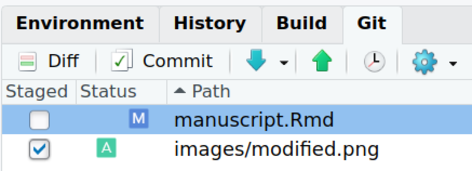
\includegraphics{/home/rstudio/images/modified.pdf}
\caption{Figure 3.1: The Git pane in R Studio, showing
\texttt{manuscript.Rmd} modified but unstaged and \texttt{modified.png}
newly added and staged.}
\end{figure}

For \texttt{Git} to recognize changes to a given file, you have to stage
and then commit these changes (this is the basic save action for a
project snapshot). One way to do this is through the visual user
interface in the RStudio \texttt{Git} pane (see Figure 3.1). Click on
the empty box next to the file you want to stage. A checkmark then
indicates that the file is staged. After you have staged all of the
files you want, click on the commit button, explain in the commit
message why you made those changes, and then click on commit. This
stores a snapshot of the current state of the project.

The files you created and the changes you made have not yet left your
computer. All snapshots are stored in a local repository in your project
folder. To back up and/or share the files online, you can push your
local repository to a remote repository. While you can choose any
\texttt{Git} service (like GitLab or BitBucket), we will use GitHub in
this tutorial. Before you upload your project to GitHub, you need to
decide whether you would like the project to be publicly accessible
(viewable by anyone, editable by selected collaborators) or if you want
to keep it private (only viewable and editable by selected
collaborators). To upload the project publicly to GitHub use:

\begin{Shaded}
\begin{Highlighting}[]
\NormalTok{usethis}\SpecialCharTok{::}\FunctionTok{use\_github}\NormalTok{()}
\end{Highlighting}
\end{Shaded}

To upload it privately:

\begin{Shaded}
\begin{Highlighting}[]
\NormalTok{usethis}\SpecialCharTok{::}\FunctionTok{use\_github}\NormalTok{(}\AttributeTok{private =} \ConstantTok{TRUE}\NormalTok{)}
\end{Highlighting}
\end{Shaded}

Depending on your computer's configuration, it may ask you to set up a
secure connection to GitHub. In this case, first, follow the suggestions
shown on the R console.

\hypertarget{using-dynamic-document-generation}{%
\subsection{Using Dynamic Document
Generation}\label{using-dynamic-document-generation}}

Now that you have created a version-controlled project, we will proceed
with dynamic document generation. A dynamic document has three elements:

\begin{enumerate}
\def\labelenumi{\arabic{enumi}.}
\tightlist
\item
  Text (prose; e.g., a scientific paper or presentation)
\item
  Executable code (e.g., analyses)
\item
  Metadata (e.g.~title, authors, document format)
\end{enumerate}

\texttt{R\ Markdown} is a type of dynamic document well-suited to the
RStudio user interface. The text of an \texttt{R\ Markdown} is formatted
by \texttt{Markdown} (see \citep{xieMarkdownDefinitiveGuide2019} for
technical details and \citep{xieMarkdownCookbook2020} for practical
guidance). The code mostly consists of R code (although other
programming languages are supported, like Python, C++, Fortran, etc).
The following example serves to illustrate the \texttt{Markdown} syntax.
It shows how to create a heading, a word in bold font, a citation, and a
list of several items in \texttt{Markdown}:

\begin{Shaded}
\begin{Highlighting}[]
\CommentTok{\textless{}!{-}{-}this is a Markdown file {-}{-}\textgreater{}}
\FunctionTok{\# Heading (level 1)}

\NormalTok{Normal text.}
\NormalTok{Important **word** in bold.}
\NormalTok{A citation: @einstein1935 did important research on this topic.}

\FunctionTok{\#\# Subheading (level 2)}

\NormalTok{To do list:}

\SpecialStringTok{* }\NormalTok{Do research}
\SpecialStringTok{* }\NormalTok{Do more research}
\SpecialStringTok{* }\NormalTok{Spend time with family and friends}
\end{Highlighting}
\end{Shaded}

One advantage of this type of markup for formatting is that it can be
rendered to many different output formats---both in terms of file types,
like \texttt{.docx}, \texttt{.html}, \texttt{.pdf}, and in terms of
style, e.g.~specific journal requirements. For social scientists, the
\href{https://github.com/crsh/papaja}{\texttt{papaja}} package
\citep{papaja} may be relevant, as it produces manuscripts that follow
the American Psychological Association formatting requirements
\citep{apa7}. \texttt{R\ Markdown} files are plain text, which is more
suitable for version control using \texttt{Git} than binary files
generated by some word processors. Some users might find it easier to
activate the ``Visual Editor'' of RStudio ({[}Ctrl{]} + {[}Shift{]} +
{[}F4{]} or click on the icon that resembles drawing materials or a
compass in the upper right corner of the \texttt{R\ Markdown} document),
which features more graphical elements like a traditional word processor
but still creates an \texttt{R\ Markdown} underneath with all of its
flexibility. The visual editor has some additional benefits, such as
promoting best practices (for example, each sentence should be written
on a new line, which makes it easier to track changes across versions)
and improving the generation of citations and references to tables and
figures.

Now that you are familiar with \texttt{Markdown} formatting basics, we
turn our attention to including code and its results in the text. Code
is separated by three backticks (and the programming language in curly
brackets) like this:

\begin{Shaded}
\begin{Highlighting}[]
\NormalTok{This is normal text, written in Markdown.}

\InformationTok{\textasciigrave{}\textasciigrave{}\textasciigrave{}\{r\}}
\InformationTok{\# this is R code}
\InformationTok{1 + 1}
\InformationTok{\textasciigrave{}\textasciigrave{}\textasciigrave{}}
\end{Highlighting}
\end{Shaded}

The hotkey {[}Control{]}+{[}Alt{]}+{[}i{]} inserts a block of code in
the file. The results of code enclosed in such backticks will be
dynamically inserted into the document (depending on specific settings).
This means that whenever you render the \texttt{R\ Markdown} to its
intended output format, the code will be executed and the results
updated. The resulting output document will be static, e.g., a pdf
document, and can be shared wherever you like, e.g., on a preprint
server.

Once the \texttt{R\ Markdown} file has been rendered to a static
document (the output, e.g., PDF), the resulting file is decoupled from
the \texttt{R\ Markdown} and the code that created it. This introduces a
risk that multiple versions of the static document are disseminated,
each with slightly different results. To avoid ambiguity, we, therefore,
recommend referencing the identifier of the \texttt{Git} commit at the
time of rendering in the static document. Simply put, a static document
should link to the version of the code that was used to create it. The
\texttt{repro} package comes with the function
\texttt{repro::current\_hash()} for this purpose. This document was
created from the commit with the hash
\href{https://github.com/aaronpeikert/repro-tutorial/tree/a8bb0d4df4afa4f7dbb5cd2344ae16043cb8a99d}{\texttt{a8bb0d4}
(view on GitHub)}.

Now that you know how to write text and R code in an
\texttt{R\ Markdown}, you need to know about metadata (also called: YAML
front matter). These metadata contain information about the document,
like the title and the output format. Metadata are placed at the
beginning of the document and are separated from the document body by
three dashes. The following example is a full markdown document where
the metadata (the ``YAML front matter'') are in lines 1--6. Some
metadata fields are self-explanatory (like the author field), and exist
across all output formats (like the title field). Others are specific to
certain output formats or R packages.

\begin{Shaded}
\begin{Highlighting}[]
\CommentTok{{-}{-}{-}}
\AnnotationTok{title:}\CommentTok{ "A Tutorial on how to Do the Same Thing More Than Once"}
\AnnotationTok{author:}\CommentTok{ Aaron Peikert, Caspar J. van Lissa, and Andreas M. Brandmaier}
\AnnotationTok{abstract:}\CommentTok{ A hitchhiker\textquotesingle{}s guide to reproducible research in R}
\AnnotationTok{output:}\CommentTok{ html\_document}
\CommentTok{{-}{-}{-}}

\FunctionTok{\# Introduction}

\NormalTok{Important for reproducibility:}

\SpecialStringTok{1. }\NormalTok{*Version control*}
\SpecialStringTok{2. }\NormalTok{*Dynamic document creation*}
\SpecialStringTok{3. }\NormalTok{*Dependency tracking*}
\SpecialStringTok{4. }\NormalTok{*Software management*}

\InformationTok{\textasciigrave{}\textasciigrave{}\textasciigrave{}\{r\}}
\InformationTok{\# this is R code}
\InformationTok{t.test(extra \textasciitilde{} group, data = sleep)}
\InformationTok{\textasciigrave{}\textasciigrave{}\textasciigrave{}}
\end{Highlighting}
\end{Shaded}

\hypertarget{manage-software-and-file-dependencies}{%
\subsection{Manage Software and File
Dependencies}\label{manage-software-and-file-dependencies}}

The \texttt{repro} package adds fields to the metadata to list all
dependencies of the research project. This includes R scripts, data
files, and external packages. The format is as follows (see everything
below the line \emph{repro:}):

\begin{Shaded}
\begin{Highlighting}[]
\CommentTok{{-}{-}{-}}
\AnnotationTok{title:}\CommentTok{ "A tutorial on how to do the same thing more than once"}
\AnnotationTok{author:}\CommentTok{ Aaron Peikert, Caspar J. Van Lissa and Andreas M. Brandmaier}
\AnnotationTok{output:}\CommentTok{ html\_document}
\AnnotationTok{repro:}
\CommentTok{  scripts:}
\CommentTok{    {-} R/load.R}
\CommentTok{  data:}
\CommentTok{    {-} data/mtcars.csv}
\CommentTok{  packages:}
\CommentTok{    {-} tidyverse}
\CommentTok{    {-} usethis}
\CommentTok{    {-} gert}
\CommentTok{{-}{-}{-}}
\end{Highlighting}
\end{Shaded}

This information clarifies what dependencies (in the form of files and R
packages) a project relies on. \texttt{repro} uses this information to
construct a \texttt{Makefile} for the dependencies on other files and a
\texttt{Dockerfile} that includes all required packages. Together, these
two files form the basis for consistency within a research project and
consistency across different systems. The function
\texttt{repro::automate()} converts the metadata from all
\texttt{R\ Markdown} files in the project (all files with the ending
\texttt{.Rmd}) to a \texttt{Makefile} and a \texttt{Dockerfile}. These
files allow users (including your future self) to reproduce every step
in the analysis automatically. Please run \texttt{repro::automate()} in
your project:

\begin{Shaded}
\begin{Highlighting}[]
\NormalTok{repro}\SpecialCharTok{::}\FunctionTok{automate}\NormalTok{()}
\end{Highlighting}
\end{Shaded}

It is important to re-run \texttt{repro::automate()} whenever you change
the \texttt{repro} metadata, change the output format, or add a new
\texttt{R\ Markdown} file to the project to keep the \texttt{Makefile}
and \texttt{Dockerfile} up to date. There is no harm in running it too
often. Other than the \texttt{Makefile} and the \texttt{Dockerfile},
which are created in the document root path, \texttt{repro} generates a
few more files in the \texttt{.repro} directory (which we will explain
in detail later), all of which you should add and commit to
\texttt{Git}.

\hypertarget{reproducing-a-project}{%
\subsection{Reproducing a project}\label{reproducing-a-project}}

If someone (including you) wants to reproduce your project, they first
have to install the required software, that is \texttt{Make}, and
\texttt{Docker}. Remember, you can use the \texttt{check\_*}-functions
to test if these are installed:

\begin{Shaded}
\begin{Highlighting}[]
\NormalTok{repro}\SpecialCharTok{::}\FunctionTok{check\_make}\NormalTok{()}
\end{Highlighting}
\end{Shaded}

\begin{verbatim}
## v Make is installed, don't worry.
\end{verbatim}

\begin{Shaded}
\begin{Highlighting}[]
\NormalTok{repro}\SpecialCharTok{::}\FunctionTok{check\_docker}\NormalTok{()}
\end{Highlighting}
\end{Shaded}

\begin{verbatim}
## v Docker is installed, don't worry.
\end{verbatim}

When these are set up, they can ask \texttt{repro} to explain how they
should use \texttt{Make} and \texttt{Docker} to reproduce the project
(or you could explain it to them):

\begin{Shaded}
\begin{Highlighting}[]
\NormalTok{repro}\SpecialCharTok{::}\FunctionTok{reproduce}\NormalTok{()}
\end{Highlighting}
\end{Shaded}

\begin{verbatim}
## * To reproduce this project, run the following code in a terminal:
\end{verbatim}

\begin{verbatim}
##   make docker &&
##   make -B DOCKER=TRUE
\end{verbatim}

If you feel uncomfortable using the terminal directly, you can send the
command to the terminal from within R:

\begin{Shaded}
\begin{Highlighting}[]
\FunctionTok{system}\NormalTok{(repro}\SpecialCharTok{::}\FunctionTok{reproduce}\NormalTok{())}
\end{Highlighting}
\end{Shaded}

The only ``hard'' software requirement for reproducing a project is
\texttt{Docker}, assuming users know how to build a \texttt{Docker}
image and run \texttt{Make} within the container. However, if they have
installed \texttt{Make} in addition to \texttt{Docker}, they do not even
need to know how to use \texttt{Docker} and can simply rely on the two
\texttt{Make} commands ``\texttt{make\ docker}'' and
``\texttt{make\ -B\ DOCKER=TRUE}''.

\hypertarget{summary}{%
\subsection{Summary}\label{summary}}

\begin{enumerate}
\def\labelenumi{\arabic{enumi}.}
\tightlist
\item
  Install the \texttt{repro} package:
\end{enumerate}

\begin{Shaded}
\begin{Highlighting}[]
\FunctionTok{options}\NormalTok{(}
  \AttributeTok{repos =} \FunctionTok{c}\NormalTok{(}\AttributeTok{aaronpeikert =} \StringTok{\textquotesingle{}https://aaronpeikert.r{-}universe.dev\textquotesingle{}}\NormalTok{,}
            \AttributeTok{CRAN =} \StringTok{\textquotesingle{}https://cloud.r{-}project.org\textquotesingle{}}\NormalTok{)}
\NormalTok{)}
\FunctionTok{install.packages}\NormalTok{(}\StringTok{\textquotesingle{}repro\textquotesingle{}}\NormalTok{)}
\end{Highlighting}
\end{Shaded}

\begin{enumerate}
\def\labelenumi{\arabic{enumi}.}
\setcounter{enumi}{1}
\tightlist
\item
  Check the required software:
\end{enumerate}

\begin{Shaded}
\begin{Highlighting}[]
\NormalTok{repro}\SpecialCharTok{::}\FunctionTok{check\_git}\NormalTok{()}
\end{Highlighting}
\end{Shaded}

\begin{verbatim}
## v Git is installed, don't worry.
\end{verbatim}

\begin{Shaded}
\begin{Highlighting}[]
\NormalTok{repro}\SpecialCharTok{::}\FunctionTok{check\_github}\NormalTok{()}
\end{Highlighting}
\end{Shaded}

\begin{verbatim}
## v You and GitHub are on good terms, don't worry.
\end{verbatim}

\begin{Shaded}
\begin{Highlighting}[]
\NormalTok{repro}\SpecialCharTok{::}\FunctionTok{check\_make}\NormalTok{()}
\end{Highlighting}
\end{Shaded}

\begin{verbatim}
## v Make is installed, don't worry.
\end{verbatim}

\begin{Shaded}
\begin{Highlighting}[]
\NormalTok{repro}\SpecialCharTok{::}\FunctionTok{check\_docker}\NormalTok{()}
\end{Highlighting}
\end{Shaded}

\begin{verbatim}
## v You are inside a Docker container!
\end{verbatim}

\begin{enumerate}
\def\labelenumi{\arabic{enumi}.}
\setcounter{enumi}{2}
\tightlist
\item
  Create an R project or use an existing one. Do not forget to add
  \texttt{repro} metadata (i.e., packages, scripts, data).
\end{enumerate}

\begin{Shaded}
\begin{Highlighting}[]
\FunctionTok{repro}\KeywordTok{:}
\AttributeTok{  }\FunctionTok{scripts}\KeywordTok{:}
\AttributeTok{    }\KeywordTok{{-}}\AttributeTok{ R/load.R}
\AttributeTok{  }\FunctionTok{data}\KeywordTok{:}
\AttributeTok{    }\KeywordTok{{-}}\AttributeTok{ data/mtcars.csv}
\AttributeTok{  }\FunctionTok{packages}\KeywordTok{:}
\AttributeTok{    }\KeywordTok{{-}}\AttributeTok{ tidyverse}
\end{Highlighting}
\end{Shaded}

The sample \texttt{repro} project already has theese metadata:

\begin{Shaded}
\begin{Highlighting}[]
\NormalTok{repro}\SpecialCharTok{::}\FunctionTok{use\_repro\_template}\NormalTok{(}\StringTok{"/some/folder"}\NormalTok{)}
\end{Highlighting}
\end{Shaded}

\begin{enumerate}
\def\labelenumi{\arabic{enumi}.}
\setcounter{enumi}{3}
\tightlist
\item
  Let \texttt{repro} generate \texttt{Docker}- and \texttt{Makefile}:
\end{enumerate}

\begin{Shaded}
\begin{Highlighting}[]
\NormalTok{repro}\SpecialCharTok{::}\FunctionTok{automate}\NormalTok{()}
\end{Highlighting}
\end{Shaded}

\begin{enumerate}
\def\labelenumi{\arabic{enumi}.}
\setcounter{enumi}{4}
\tightlist
\item
  Enjoy automated reproducibility:
\end{enumerate}

\begin{Shaded}
\begin{Highlighting}[]
\NormalTok{repro}\SpecialCharTok{::}\FunctionTok{reproduce}\NormalTok{()}
\end{Highlighting}
\end{Shaded}

\begin{verbatim}
## * To reproduce this project, run the following code in a terminal:
\end{verbatim}

\begin{verbatim}
##   make docker &&
##   make -B DOCKER=TRUE
\end{verbatim}

\hypertarget{advanced-features}{%
\section{Advanced Features}\label{advanced-features}}

This section is for advanced users who want to overcome some limitations
of \texttt{repro}. If you read this paper the first time, you will
probably want to skip this section and continue reading from the section
``Preregistration as Code.'' As explained above, \texttt{repro} is
merely a simplified interface to the tools that enable reproducibility.
This simplified interface imposes two restrictions. Users who ask
themselves either, ``How can I install software dependencies outside of
R in the \texttt{Docker} image?'' or ``How can I express complex
dependencies between files (e.g., hundreds of data files are
preprocessed and combined)?'' need to be aware of these restrictions and
require a deeper understanding of the inner workings of \texttt{repro}.
Other users may safely skip this section or return to it if they
encounter such challenges.

The first restriction is that users must rely on software that is either
already provided by the base \texttt{Dockerimage} ``rocker/verse'' or
the R packages they list in the metadata. The metadata the
\texttt{repro::automate()} function relies on can only express R
packages as dependencies for the \texttt{Dockerfile} and only trivial
dependencies (in the form of ``file must exist'') for the
\texttt{Makefile}. Other software that users might need, like other
programming languages, not yet installed LaTeX packages, etc., must be
added manually. We plan to add support for commonly used ways to install
software beyond R packages via the metadata and
\texttt{repro::automate()}, for example, for system libraries (via
\texttt{apt} the Ubuntu package manager), LaTeX packages (via
\texttt{tlmgr} the Tex Live package manager), Python packages (via
\texttt{pip} the python package manager). The second limitation is
related to dependencies. \texttt{Make} can represent complex
dependencies, for example: A depends on B, which in turn depends on C
and D. If B is missing in this example, \texttt{Make} would know how to
recreate it from C and D. These dependencies, and how they should be
resolved, are difficult to represent in the metadata. Users, therefore,
have to either ``flatten'' the dependency structure by simply stating
that A depends on B, C, and D, thereby leaving out important information
or express the dependencies directly within the \texttt{Makefile}.

The following section explains how to overcome these limitations despite
reliance on the automation afforded by \texttt{repro}. Lifting these
restrictions requires the user to interact more directly with
\texttt{Make} or \texttt{Docker}. Users need to understand how repro
utilizes \texttt{Make} and \texttt{Docker} internally to satisfy more
complicated requirements.

Let us have a closer look at the command for reproducing a repro
project: \texttt{make\ docker\ \&\&\ make\ -B\ DOCKER=TRUE}; which
consists of two processing steps. First, it recreates the virtual
software environment (\texttt{Docker}), and then it executes
computational recipes in the virtual software environment
(\texttt{Make}). The first step is done by the command
\texttt{make\ docker}. The command \texttt{make\ docker} will trigger
\texttt{Make} to build the target called \texttt{docker}. The recipe for
this target builds an image from the \texttt{Dockerfile} in the
repository. The \texttt{\&\&} concatenates both commands and only runs
the second command if the first is successful. Therefore, the
computational steps are only executed when the software environment is
set up. The second step executes the actual reproduction and is again a
call to \texttt{Make} in the form of \texttt{make\ -B\ DOCKER=TRUE} with
three noteworthy parts. First, a call to \texttt{make} without any
explicit target will build the \texttt{Make} target \texttt{all}.
Second, the flag \texttt{-B} means that \texttt{Make} will consider all
dependencies as outdated and will hence rebuild everything. Third, repro
constructs \texttt{Make} targets so that if you supply
\texttt{DOCKER=TRUE} they are executed within the \texttt{Docker} image
of the project.

The interplay between \texttt{Docker} and \texttt{Make} resembles a
chicken or egg problem. We have computational steps (\texttt{Make}) that
depend on the software environment (\texttt{Docker}) for which we again
have computational steps that create it. Users only require a deeper
understanding of this interdependence when they either want to have more
complex computational recipes than rendering an \texttt{R\ Markdown} or
require other software than R packages.

Users can have full control over the software installed within the image
of the project. \texttt{repro} creates three \texttt{Dockerfiles} inside
the \texttt{.repro} directory. Two \texttt{Dockerfiles} are
automatically generated. The first is \texttt{.repro/Dockerfile\_base}.
It contains information about the base image on which all the remaining
software is installed. By default we rely on the ``verse'' images
provided by the Rocker project
\citep{boettigerIntroductionRockerDocker2017}. These contain (among
other software) the packages \texttt{tidyverse}, \texttt{rmarkdown}, and
a complete LaTeX installation, which makes these images ideal for the
creation of scientific manuscripts. Users can choose which R version
they want to have inside the container by changing the version number in
line 1 to the desired R version number. By default, the R version
corresponds to the locally installed version on which
\texttt{repro::automate()} was called the first time. The build date is
used to install packages in the version that was available on the
Comprehensive R Archive Network on this specific date and can also be
changed. By default, this date is set to the date on which
\texttt{repro::automate()} was called the first time. This way, the call
to the automate function virtually freezes the R environment to the
state it was called the first time inside the container. Below, you see
the \texttt{Docker} base file we used to create this manuscript:

\begin{Shaded}
\begin{Highlighting}[]
\ExtensionTok{FROM}\NormalTok{ rocker/verse:4.0.4}
\ExtensionTok{ARG}\NormalTok{ BUILD\_DATE=2021{-}05{-}06}
\ExtensionTok{WORKDIR}\NormalTok{ /home/rstudio}
\end{Highlighting}
\end{Shaded}

The second automatically generated \texttt{Dockerfile} is
\texttt{.repro/Dockerfile\_packages}. Whenever
\texttt{repro::automate()} is called, \texttt{repro} gathers all R
packages from all \texttt{.Rmd} files and determines whether they should
be installed from CRAN or GitHub fixed to the date specified in
\texttt{Dockerfile\_base}. Finally, there is one manually edited
\texttt{Dockerfile}: \texttt{.repro/Dockerfile\_manual}. It is blank by
default and can be used to add further dependencies outside of R, like
system libraries or external software. Using \texttt{Docker} may require
you to install software on an operating system that may not be familiar
to you. The images supplied by
\citep{boettigerIntroductionRockerDocker2017}, for example, are based on
the Ubuntu operating system. The most convenient way to install software
on Ubuntu is through its package manager \texttt{apt}. If the following
snippet is added to \texttt{.repro/Dockerfile\_manual}, the
\texttt{Docker} image will have, for example, Python installed. Other
software is installed identically, only the software name is exchanged.

\begin{Shaded}
\begin{Highlighting}[]
\ExtensionTok{RUN}\NormalTok{ apt{-}get update }\KeywordTok{\&\&} \ExtensionTok{apt{-}get}\NormalTok{ install }\AttributeTok{{-}y}\NormalTok{ python3}
\end{Highlighting}
\end{Shaded}

\texttt{Docker} eventually requires a single \texttt{Dockerfile} to run,
so \texttt{repro::automate()} simply concatenates the three
\texttt{Dockerfiles} and saves the result into the main
\texttt{Dockerfile} at the top level of the R project. With this
approach, users of \texttt{repro} can build complex software
environments and implement complex file dependencies. The standard
\texttt{repro} metadata only make sure that all dependencies are
available but does not allow you to specify custom recipes for them in
the metadata. If you can formulate the creation of dependencies in terms
of computational steps, e.g.~the file \texttt{data/clean.csv} is created
from \texttt{data/raw.csv} by script \texttt{R/preprocess.R}, you should
include these in the \texttt{Makefile}. The \texttt{Makefile} that
\texttt{repro} creates is only a template, and you are free to change
it. However, make sure you never remove the following two lines:

\begin{Shaded}
\begin{Highlighting}[]
\ExtensionTok{include}\NormalTok{ .repro/Makefile\_Rmds}
\ExtensionTok{include}\NormalTok{ .repro/Makefile\_Docker}
\end{Highlighting}
\end{Shaded}

The file \texttt{.repro/Makefile\_Rmds} contains the automatically
generated targets from \texttt{repro::automate()} for the
\texttt{R\ Markdown} files. This file should not be altered manually. If
you are not satisfied with the automatically generated target, simply
provide an alternative target in the main \texttt{Makefile}. Targets in
the main \texttt{Makefile} take precedent.

The file \texttt{.repro/Makefile\_Docker} does again contain a rather
complicated template that you could, but should usually not modify. This
\texttt{Makefile} coordinates the interplay between \texttt{Make} and
\texttt{Docker} and contains targets for building (with
\texttt{make\ docker}) and saving (with \texttt{make\ save-docker}) the
\texttt{Docker} image. Additionally, it provides facilities to execute
commands within the container. If you write a computational recipe for a
target, it will be evaluated using the locally installed software by
default. To evaluate commands inside the \texttt{Docker} image instead,
you should wrap them in \texttt{\$(RUN1)\ command\ \$(RUN2)}, as done in
this example, which is identical to the first \texttt{Make} example we
gave above except for the addition of \texttt{\$(RUN1)} and
\texttt{\$(RUN2)} in l. 2:

\begin{Shaded}
\begin{Highlighting}[]
\ExtensionTok{simulated\_data.csv:}\NormalTok{ R/simulate.R}
  \VariableTok{$(}\ExtensionTok{RUN1}\VariableTok{)}\NormalTok{ Rscript }\AttributeTok{{-}e} \StringTok{\textquotesingle{}source("R/simulate.R")\textquotesingle{}} \VariableTok{$(}\ExtensionTok{RUN2}\VariableTok{)}
\end{Highlighting}
\end{Shaded}

If users execute this in the terminal:

\begin{Shaded}
\begin{Highlighting}[]
\FunctionTok{make}\NormalTok{ data/simulation\_results.csv}
\end{Highlighting}
\end{Shaded}

It behaves exactly as in the first \texttt{Make} example, the script
\texttt{R/simulate.R} is run using the locally installed R. Because this
translates simply to:

\begin{Shaded}
\begin{Highlighting}[]
\ExtensionTok{Rscript} \AttributeTok{{-}e} \StringTok{\textquotesingle{}source("R/simulation.R")\textquotesingle{}}
\end{Highlighting}
\end{Shaded}

But if users use

\begin{Shaded}
\begin{Highlighting}[]
\FunctionTok{make}\NormalTok{ DOCKER=TRUE data/simulation\_results.csv}
\end{Highlighting}
\end{Shaded}

it is evaluated within the \texttt{Docker} container using the software
within it and not the locally installed R version:

\begin{Shaded}
\begin{Highlighting}[]
\ExtensionTok{docker}\NormalTok{ run }\AttributeTok{{-}{-}rm} \AttributeTok{{-}{-}user}\NormalTok{ 1000 }\AttributeTok{{-}v} \StringTok{"/home/rstudio"}\NormalTok{:}\StringTok{"/home/rstudio/"}
\ExtensionTok{reprotutorial}\NormalTok{ Rscript }\AttributeTok{{-}e} \StringTok{\textquotesingle{}source("R/simulate.R")\textquotesingle{}}
\end{Highlighting}
\end{Shaded}

To summarize, \texttt{repro} automates dependency tracking (in the form
of \texttt{Make}) and software management (using \texttt{Docker})
without the necessity to learn both tools, but users with advanced
requirements can still customize all aspects of both programs.

\hypertarget{preregistration-as-code}{%
\section{Preregistration as Code}\label{preregistration-as-code}}

\emph{Preregistration} refers to the practice of defining research
questions and planning data analysis before observing the research
outcomes \citep{NosekRevolution2018}. It serves to separate a-priori
planned and theory-driven (confirmatory) analyses from unplanned and
post-hoc (exploratory) analyses. Researchers are faced with a myriad of
choices in designing, executing, and analyzing a study, often called
researchers degrees of freedom. Undisclosed researcher degrees may be
used to modify planned analyses until a key finding reaches statistical
significance or to inflate effect size estimates, a phenomenon referred
to as \emph{opportunistic bias}
\citep{decosterOpportunisticBiasesTheir2015}. Preregistration increases
transparency by clarifying when and how researchers employ their degrees
of freedom. It expressly does not restrict what researchers may do to
gather or analyze their data.

There are still several shortcomings to preregistration. One is that
written study plans are often interpretable in multiple ways. Empirical
research has shown that, even when several researchers describe their
analysis with the same terms, use the same data, and investigate the
same hypothesis, their results vary considerably
\citep{silberzahnManyAnalystsOne2018}. The current best practice to
ensure comprehensive and specific preregistration is to impose structure
by following preregistration templates
\citep{bowmanOSFPreregTemplate2020, bakkerEnsuringQualitySpecificity2020}.
However, such templates cannot ensure full transparency because it is
impossible to verbally describe every detail of an analysis for any but
the most straightforward analysis. This ambiguity causes a second
problem, namely, comparing the initial plan and the resulting
publication to decide if and how researchers deviated from the
preregistration. This task is difficult because it is impossible to
decide without additional information weather the analysis was actually
carried out differently or just described differently. Even if
researchers were faithful to the preregistration, readers may reach
opposite conclusions because they have to compare two different text
that may be worded differently or describe the same thing in varying
levels of detail. A third limitation is that preregistrations are
susceptible to non-reproducibility, just like primary research. To
illustrate, a review of 210 preregistrations found that, even though 174
(67\%) included a formal power analysis, only 34 (20\%) of these could
be reproduced \citep{bakkerRecommendationsPreregistrationsInternal2020}.
Even when researchers have gone to great lengths in preregistering an
analysis script, they sometimes inexplicably fail to reproduce their own
results. For example, \citet{steegenMeasuringCrowdAgain2014} realized
after publication that part of their preregistered code resulted in
different test statistics than they reported initially (see their
Footnote 7). A final limitation is that written plans may turn out to be
unfeasible once data are obtained and analyzed. For example, a verbal
description of a statistical model may be unidentified, e.g., if it
includes reciprocal paths between variables or more parameters than
observed data. Conversely, a model may be misspecified in a major way;
for example, by omitting direct effects when the research question is
about mediation, thus leading to a model with an unacceptable fit. Many
researchers would only realize that such a model cannot be estimated
once the data are obtained, thus necessitating a deviation from the
preregistered plans.

The workflow described in this paper facilitates a rigorous solution to
this problem: Instead of describing the analysis in prose, researchers
include the code required to conduct the analysis in the
preregistration. We term this approach of writing and publishing code at
the preregistration stage \emph{Preregistration as Code (PAC)}. PAC has
the potential to eliminate undisclosed researchers degrees of freedom to
a much greater extent than, e.g., preregistration templates. Moreover,
it reduces overhead by removing the need to write a separate
preregistration and manuscript. For PAC, researchers can write a
reproducible, dynamically generated draft of their intended manuscript
at the preregistration stage. This already includes most of the typical
sections, such as introduction, methods, and results. These results are
initially based on simulated data with the same structure as the data
the authors expect to obtain from their experiments. For guidance on how
to simulate data, see \citet{morrisUsingSimulationStudies2019},
\citet{paxtonMonteCarloExperiments2001}, and
\citet{skrondalDesignAnalysisMonte2000}, as well as the R packages
\href{https://cran.r-project.org/web/packages/simstudy/vignettes/simstudy.html}{\texttt{simstudy}},
\citep{simstudy} and
\href{https://personality-project.org/r/psych/help/sim.html}{\texttt{psych}},
\citep{psych}.

Once the preregistration is submitted and real data have been collected
or made available, the document can be reproduced with a single command,
thus updating the Results section to the final version. Reproducibility
is of utmost importance at this stage since the preregistration must
produce valid results at two points in time, once before data collection
and once after data collection. As outlined before, reproducibility
builds upon four pillars (version control, dynamic document generation,
dependency tracking, and software management). To use PAC the dangers to
reproducibility we described must be eliminated.

The idea of submitting code as part of a preregistration is not new
\citep[e.g.][]{wichertsDegreesFreedomPlanning2016}. A prominent
preregistration platform, \href{https://osf.io/}{The Open Science
Framework}, suggests submitting scripts alongside the preregistration of
methods. In an informal literature search (we skimmed the first 300
results of Google Scholar with the keywords
\texttt{("pre\ registration"\textbar{}"pre-registration"\textbar{}preregistration)\&(code\textbar{}script\textbar{}matlab\textbar{}python\textbar{}"R")})
we only found close to a dozen published articles that did include some
form of script as part of their preregistration. Though the notion of
preregistering code has been around for a while
\citep[cf.][]{steegenMeasuringCrowdAgain2014}, it has not gained much
traction---perhaps because, to date, this has constituted an extra
non-standard step in the research process. This tutorial integrates the
preregistration of code into the reproducible research workflow by
encouraging researchers to preregister the whole manuscript as a dynamic
document.

\hypertarget{advantages-of-pac-over-traditional-preregistration}{%
\subsection{Advantages of PAC Over Traditional
Preregistration}\label{advantages-of-pac-over-traditional-preregistration}}

We believe that pairing PAC with the workflow presented above offers
five advantages over classical preregistration. First, PAC is merely an
intermediate stage of the final manuscript, thus sparing authors from
writing, and editors and reviewers from evaluating, two separate
documents. Relatedly, writing the preregistration in the form of a
research article has the advantage that researchers are usually familiar
with this format. By contrast, a preregistration template is a novelty
for many. Second, PAC is a tool for study planning. A study can be
carried out more efficiently if all steps are documented clearly than
when every step is planned ad hoc. Third, PAC removes ambiguity
regarding the translation of verbal analysis plans into code. PAC is
more comprehensive by design because its completeness can be empirically
checked with simulated data. Evaluating the intended analysis code on
simulated data will help identify missing steps or ambiguous decisions.
PAC, therefore, minimizes undisclosed researchers degrees of freedom
more effectively than standard preregistration does
\citep{bakkerEnsuringQualitySpecificity2020, wichertsDegreesFreedomPlanning2016}.
Fourth, despite its rigor, PAC accommodates data-dependent decisions if
these can be formulated as code. Researchers can, for example, formulate
conditions (e.g., in the form of if-else-blocks) under which they prefer
one analysis type over the other. For example, if distributional
assumptions are not met, the code may branch out to employ robust
methods; or, an analysis may perform automated variable selection
mechanisms before running the final model. Another example of
data-dependent decisions are more explorative analyses, i.e.~explorative
factor analysis or machine learning. Decisions that do not lend
themselves to formulation in code, e.g.~visual inspection, must still be
described verbally or be treated as noted in the next section. Fifth,
deviations from the preregistration are clearly documented because they
are reflected in changes to the code, which are managed and tracked with
version control.

\hypertarget{deviating-from-the-preregistration-and-exploration}{%
\subsection{Deviating from the Preregistration and
Exploration}\label{deviating-from-the-preregistration-and-exploration}}

We would like to note that PAC allows explicit comparison of the
preregistration and the final publication. Authors should
retrospectively summarize and justify any changes made to the
preregistered plan, e.g.~in the discussion of the final manuscript
\footnote{In section {[}Preregistration as Code --- a Tutorial{]} we
  conducted an actual PAC and summarize the changes we make to the
  preregistered code in the discussion.}. During the analysis process,
authors can additionally maintain a running changelog to explain changes
in detail as they arise. Each entry in the changelog should explain the
reasoning behind the changes and link to the commit id that applied the
changes. This enables readers and reviewers to inspects individual
changes and make an informed judgment about their validity and
implications.

Deviations from the preregistration are sometimes maligned, as if
encountering unexpected challenges invalidates a carefully crafted study
\citep{szollosi_is_2020}. However, we share the common view that
deviation from a preregistration is not a problem
\citep{nosekPreregistrationHardWorthwhile2019}; rather, a faillure to
disclose such deviations is a problem. In fact, it is expected that most
PACs will require some modification after empirical data becomes
available. Often, deviations provide an opportunity to learn from the
unexpected.

For example, imagine that authors preregistered their intention to
include both ``working memory'' and ``fluid intelligence'' as covariates
in an experimental study, examining the effect of task novelty on
reaction time. When evaluating the planned analyses on the empirical
data, these two covariates reveal high collinearity, thus compromising
statistical inference. The authors decide to use PCA to extract common
variance related to ``intelligence'', and include this component as a
covariate instead. This change pertains to an auxiliary assumption (that
working memory and fluid intelligence are distinct constructs), but does
not undermine the core theory (that task novelty affects reaction time).
Now imagine that a different researcher is interested in the structure
of intelligence. This change to the preregistration directly relates to
their theory of intelligence. That researcher might thus interpret the
same result as an explorative finding, suggesting that these aspects of
intelligence are unidimensional. A deviation from preregistration thus
requires a judgement about what changes affect the test of the theory to
what extend \citep{meehlTheoreticalRisksTabular1978}. Only transparent
reporting enables such judgment.

Another common misunderstanding is that preregistration, including PAC,
precludes exploratory analyses. We differentiate between two kinds of
exploration, neither of which is limited by PAC. The first, more
traditional kind of exploration involves ad hoc statistical decisions
and post hoc explanations of the results. Such traditional exploratory
findings should be explicitly declared in the manuscript to distinguish
them from confirmatory findings
\citep{NosekRevolution2018, nosekPreregistrationHardWorthwhile2019}. The
second kind of exploration is through procedurally well defined
exploration with exploratory statistical models that are standard in
machine learning \citep{brandmaier22mlsem}. These models often involve
dozens, if not hundreds of predictors, which makes it difficult to
describe them verbally. With PAC, such models can be preregistered
clearly and in comprehensive detail and researcher can precisely define
a priori how much they want to explore. We specifically recommend PAC
for such exploratory statistical models. The merit of preregistration in
these cases is to communicate precisely how much exploration was done; a
piece of information that is crucial to assess e.g., whether the results
might be overfit
\citep[p.~220f.]{hastieElementsStatisticalLearning2017}.

\hypertarget{planned-analyses-as-functions}{%
\subsection{Planned Analyses as
Functions}\label{planned-analyses-as-functions}}

Although researchers may use any form to preregister their planned
analyses (e.g., scripts), we suggest writing three functions for each
planned hypothesis: one to conduct the planned analysis, one to simulate
the expected data, and to report the results. Using functions makes the
analysis more portable (i.e., it can easily be used for other datasets),
and facilitates repeated evaluation, as is the case in a simulation
study. The functions shown here do not contain executable code, but the
interested reader can find working functions in the
\href{https://github.com/aaronpeikert/repro-tutorial/blob/main/R/simulation_funs.R}{online
supplementary materials} that power the example below.

It is difficult to write analysis code when it is not clear what the
expected data will look like. We therefore recommend first simulating a
dataset that resembles the expected structure of the empirical data that
will be used for the final analysis. Dedicated packages to simulate data
for specific analyses exist .

The general format of a simulation function might be as follows:

\begin{Shaded}
\begin{Highlighting}[]
\NormalTok{simulate\_data }\OtherTok{\textless{}{-}} \ControlFlowTok{function}\NormalTok{(n, effect\_size)\{}
  \CommentTok{\# 1. warn users that the results are "fake"}
  \CommentTok{\# 2. draw \textasciigrave{}n\textasciigrave{} samples with \textasciigrave{}effect\_size\textasciigrave{}}
  \CommentTok{\# 3. format and return in expected data format}
\NormalTok{\}}
\end{Highlighting}
\end{Shaded}

For linear models, simulating data is extremely simple:

\begin{Shaded}
\begin{Highlighting}[]
\NormalTok{simulate\_data }\OtherTok{\textless{}{-}} \ControlFlowTok{function}\NormalTok{(n, effect\_size)\{}
  \FunctionTok{warning}\NormalTok{(}\StringTok{"This manuscript contains mock results based on simulated data."}\NormalTok{)}
  \CommentTok{\# Draw n samples from a normal distribution for predictor X}
\NormalTok{  x }\OtherTok{\textless{}{-}} \FunctionTok{rnorm}\NormalTok{(n)}
  \CommentTok{\# Calculate dependent variable Y..}
  \CommentTok{\#.. as a function of population effect size and residual error}
\NormalTok{  y }\OtherTok{\textless{}{-}}\NormalTok{ effect\_size }\SpecialCharTok{*}\NormalTok{ x }\SpecialCharTok{+} \FunctionTok{rnorm}\NormalTok{(n)}
  \CommentTok{\# Return a data.frame}
  \FunctionTok{data.frame}\NormalTok{(}\AttributeTok{x =}\NormalTok{ x, }\AttributeTok{y =}\NormalTok{ y)}
\NormalTok{\}}
\end{Highlighting}
\end{Shaded}

Next, write a function to conduct the planned analysis. This function
should receive the data and compute all relevant results from it. The
general format of an analysis function might be:

\begin{Shaded}
\begin{Highlighting}[]
\NormalTok{planned\_analyis }\OtherTok{\textless{}{-}} \ControlFlowTok{function}\NormalTok{(data)\{}
  \CommentTok{\# 1. preprocess e.g. with \textasciigrave{}rowMeans(data)\textasciigrave{}}
  \CommentTok{\# 2. conduct analysis e.g. with \textasciigrave{}t.test()\textasciigrave{}}
  \CommentTok{\# 3. \textasciigrave{}return(results)\textasciigrave{}}
\NormalTok{\}}
\end{Highlighting}
\end{Shaded}

In the simplest case, an analysis function might already exist in R. For
the linear model above, the analysis function might be:

\begin{Shaded}
\begin{Highlighting}[]
\NormalTok{planned\_analyis }\OtherTok{\textless{}{-}} \ControlFlowTok{function}\NormalTok{(data)\{}
    \FunctionTok{lm}\NormalTok{(y }\SpecialCharTok{\textasciitilde{}}\NormalTok{ x, }\AttributeTok{data =}\NormalTok{ data)}
\NormalTok{\}}
\end{Highlighting}
\end{Shaded}

As soon as we have written \texttt{planned\_anaylsis()} and
\texttt{simulate\_data()} we can iteratively improve both functions,
e.g.~until \texttt{planned\_analysis()} runs without error and recovers
the correct parameters from \texttt{simulate\_data()}. The goal is to
ensure that the output of \texttt{simulate\_data()} works as input to
the function \texttt{planned\_analysis()}.

When the researchers are satisfied with the function
\texttt{planned\_analysis()}, they can think about the way the would
they would like to report the analysis results via tables, plots, and
text. The implementation of this reporting should be in the function
\texttt{report\_analysis()}.

\begin{Shaded}
\begin{Highlighting}[]
\NormalTok{report\_analysis }\OtherTok{\textless{}{-}} \ControlFlowTok{function}\NormalTok{(results)\{}
  \CommentTok{\# 1. create markdown tables from results}
  \CommentTok{\# 2. conditionally interpret results e.g. if(p \textless{} .025)"Result is significant."}
  \CommentTok{\# (optional) visualize results}
  \CommentTok{\# 3. return results section formatted in markdown}
\NormalTok{\}}
\end{Highlighting}
\end{Shaded}

This function should again accept the output of
\texttt{planned\_analysis()} as input. The output of this function
should be formatted in Markdown. The idea is to automatically generate
the full results section from the analysis. This way, the
preregistration not only specifies the computation but also how the its
results are reported. Various packages automatically generate
well-formatted Markdown outputs of statistical reports or even entire
tables of estimates or figures directly from R goal to help with this
objective. Packages like
\href{https://github.com/Rapporter/pander}{\texttt{pander}}
\citep{pander},
\href{https://cran.r-project.org/web/packages/stargazer/vignettes/stargazer.pdf}{\texttt{stargazer}}
\citep{stargazer},
\href{https://dstanley4.github.io/apaTables/articles/apaTables.html}{\texttt{apaTables}}
\citep{apaTables} and
\href{http://frederikaust.com/papaja_man/}{\texttt{papaja}}
\citep{papaja} help you to create dynamically generated professional
looking results. The package
\href{https://github.com/easystats/report}{\texttt{report}}
\citep{report} is particularly noteworthy because it not only generates
tables but also a straightforward interpretation of the effects as
actual prose (e.g., it verbally quantifies the size of an effect).

Ideally, these three functions can be composed to create a ``fake''
results section, e.g.~when composed to
\texttt{report\_analysis(planned\_analysis(simulate\_data()))} or
\texttt{simulate\_data()\ \%\textgreater{}\%\ planned\_analysis()\ \%\textgreater{}\%\ report\_analysis()}
outputs a results section.

\hypertarget{turning-a-dynamic-document-into-a-preregistration}{%
\subsubsection{Turning a Dynamic Document into a
Preregistration}\label{turning-a-dynamic-document-into-a-preregistration}}

After researchers are satisfied with their draft preregistration, they
should archive a time-stamped and uneditable version of the project that
serves as the preregistration. zenodo.org \citep{zenodo} is a publicly
funded service provider that archives digital artefacts for research and
provides digital object identifiers (DOI) for these archives. While the
service is independent of GitHub---in terms of storage facilities and
financing---you can link GitHub and zenodo.org. Please note that you can
only link public GitHub repositories to zenodo.org. You may log into
zenodo.org through your GitHub account. To log in with your GitHub
account:

\begin{quote}
Navigate to \url{https://zenodo.org/login/} → Log in with GitHub
\end{quote}

\noindent{}To link zenodo.org and GitHub

\begin{quote}
Log into zenodo.org → Account → GitHub\footnote{\url{https://zenodo.org/account/settings/github/}}
\end{quote}

\noindent{}Or:

\begin{quote}
Navigate to \url{https://zenodo.org/account/settings/github/}
\end{quote}

After you have linked a GitHub repository, you trigger the archival by
creating a GitHub release. To create GitHub release, navigate to GitHub:

\begin{Shaded}
\begin{Highlighting}[]
\NormalTok{usethis}\SpecialCharTok{::}\FunctionTok{browse\_github}\NormalTok{()}
\end{Highlighting}
\end{Shaded}

Then click on Releases → Draft a new release. Here you can add all
relevant binary files but at least a rendered version of the manuscript
and the Docker image.

To summarize, researchers need to write three functions,
\texttt{planned\_analysis()}, \texttt{simulate\_data()}, and
\texttt{report\_analysis()} and embed these into a manuscript that
serves as a preregistration in an uneditable online repository. After
they gathered the actual data, they can replace the simulated data,
render the dynamic manuscript (therefore run
\texttt{planned\_analysis()} on the actual data), and write the
discussion.

\hypertarget{alternatives-to-simulated-data}{%
\subsection{Alternatives to simulated
data}\label{alternatives-to-simulated-data}}

Simulating data may prove challenging to applied researchers. In the
spirit of team science and collaboration, one feasible solution is to
involve a statistical co-author. However, several easy alternatives
exist. The downside of these alternatives is that they all rely
indirectly on the use of real data. This introduces a risk that the
planned analyses may be cross-contaminated by any exploratory findings.
It is crucial to disclose any exposure to the data in preparation of the
preregistration (PAC or otherwise). This exposure to the data may
decrease trust in the objectivity of the preregistration. Moreover,
researchers should take rigorous measures to prevent exposure to
exploratory findings that may unintentionally influence their decision
making.

The simplest method is to collect empirical data first, but set it aside
and proceed with a copy of the data that is blinded by randomly
shuffling the order of rows for each variable (independently of each
other). Shuffling removes any associations between variables, while
retaining information about the level of measurement and marginal
distribution of each variable. If the hypotheses pertain to associations
between variables, this treatment should thus be sufficient to prevent
cross-contamination. The researcher can still access the information
about means or proportions (e.g., the number of participants belonging
to group ``A'' are in the dataset), but remain uninformed about
relations between variables (e.g., members of group ``A'' have a greater
mean in variable ``Z''). Preregistration after data collection is common
for secondary data analysis of data obtained by other research groups
\citep{westonRecommendationsIncreasingTransparency2019} but not so much
within the same research project. We argue that it is still an eligible
preregistration. Guidelines for clinical trials already recommend
analysis of blinded data to test the feasibility of a preregistration
\citep{ICH1998}.

Another alternative to simulated data is to conduct a pilot study
\citep{thabaneTutorialPilotStudies2010} and use the pilot data to
develop the preregistration. A pilot study has obvious advantages for
study planning, since it lets the researcher evaluate the feasibility of
many assumptions. However, we must warn our readers, that while piloting
is more traditional than our approach of blinding the data before
preregistration, the data from the pilot study must not enter the
analysis data set.

\hypertarget{when-is-pac-applicable}{%
\subsection{When Is PAC Applicable?}\label{when-is-pac-applicable}}

PAC is applicable to every study that can be preregistered and
ultimately uses computer code for the statistical analysis. Two types of
preregistrations are particularly amenable to PAC. First, pregistrations
of clinical trials (called statistical analysis plans, \citet{ICH1998})
typically describe analyses in exhaustive detail and typically contain a
detailed description of how results will be presented, including shells
of tables and graphics \citep{yuanGuideStatisticalAnalysis2019}. PAC may
significantly reduce the required workload while maintaining (and
exceeding) the required standards for preregistering a clinical trial.

Second, preregistering exploratory statistical models (i.e., those with
large numbers of competing models or those inspired by machine learning)
is hardly feasible with standard preregistrations since they are too
complex to describe and depend strongly on their software
implementation. PAC, however, captures the precise algorithmic model,
including its software implementation and is ideal for preregistering
these models \citep{brandmaier22mlsem}.

\hypertarget{preregistration-as-code-tutorial}{%
\subsection{Preregistration as Code:
Tutorial}\label{preregistration-as-code-tutorial}}

We have argued that PAC has several advantages over classic
preregistration and have outlined its implementation. To illustrate how
PAC works in practice and help researchers to implement PAC themselves,
we provide a worked example. We will use an exemplary research question
that was based on openly available data:

\begin{quote}
``Is there a mean difference in the personality trait `Machiavellism'
between self-identified females and males?''
\end{quote}

Again, we propose a preregistration format that closely resembles a
classic journal article but uses simulated data and dynamic document
generation to create a document that starts out as a preregistration and
eventually becomes the final report. The complete preregistration source
is available in the
\href{https://github.com/aaronpeikert/repro-tutorial/blob/main/preregistration.Rmd}{online
supplementary material}. In this section, we show code excerpts of this
preregistration (formatted in monospace) and explain the rationale
behind them.

As usual, the authors state why they are interested in their research
question in the ``Introduction'' section and provide the necessary
background information and literature to understand the context and
purpose of the research question. This example is drastically shortened
for illustration purposes:

\begin{Shaded}
\begin{Highlighting}[]
\FunctionTok{\# Theoretical Background}

\NormalTok{Machiavellianism describes a personality dimension characterized by a}
\NormalTok{cynical disregard of morals in the pursuit of one\textquotesingle{}s own interest, e.g.}
\NormalTok{through manipulation }\CommentTok{[}\OtherTok{@christie1970}\CommentTok{]}\NormalTok{. There is extensive literature reporting}
\NormalTok{differences in the dark triad (narcissism, machiavellianism, and psychopathy)}
\NormalTok{between self{-}identified males and females }\CommentTok{[}\OtherTok{@muris2017}\CommentTok{]}\NormalTok{ but only few studies}
\NormalTok{focus solely on machiavellianism. We aim to replicate the finding that males}
\NormalTok{tend to have higher machiavellianism scores }\CommentTok{[}\OtherTok{@muris2017}\CommentTok{]}\NormalTok{.}
\end{Highlighting}
\end{Shaded}

After researchers have provided the research question, they typically
proceed to explain how they want to study it. For simplicity, we will
use already published data that we have not yet analyzed:

\begin{Shaded}
\begin{Highlighting}[]
\FunctionTok{\# Method}

\NormalTok{We report how we determined our sample size, all data exclusions (if any), all}
\NormalTok{manipulations, and all measures in the study }\CommentTok{[}\OtherTok{cf. @simmons2012}\CommentTok{]}\NormalTok{. We use data}
\NormalTok{available from }\CommentTok{[}\OtherTok{openpsychometrics.org}\CommentTok{](https://openpsychometrics.org/\_rawdata/)}
\NormalTok{from the online version of the MACH{-}IV}\CommentTok{[}\OtherTok{@christie1970}\CommentTok{]}\NormalTok{ and included participants}
\NormalTok{that have responded to at least one machiavellianism item and reported their}
\NormalTok{gender as either "male" or "female".}
\end{Highlighting}
\end{Shaded}

We choose the following statistical procedure because many researchers
are familiar with it\footnote{The t-test and Mann-Whitney-Wilcoxon test
  are arguably the most often used hypothesis tests (according to
  \citep{fagerlandTtestsNonparametricTests2012, hortonStatisticalMethodsJournal2005}
  reports that 26\% of all studies employed a t-test and 27\% employed a
  rank-based alternative in the \emph{New England Journal of Medicine}
  in 2005). The analytical strategy presented here is, in fact,
  suboptimal in several respects (the assumption of measurement
  invariance is untested
  \citep{putnickMeasurementInvarianceConventions2016}, the effect size
  is underestimated in the presence of measurement error
  \citep{frostCorrectingRegressionDilution2000}, the effect size is
  overestimated for highly skewed distributions
  \citep{stonehouseRobustnessTestsCombined1998}). The interested reader
  can use the
  \href{https://github.com/aaronpeikert/repro-tutorial/blob/main/R/simulation.R}{provided
  code for the simulation} to verify that the t-test provides unbiased
  effect sizes but the Mann-Whitney-Wilcoxon overestimates effect sizes
  with increasing sample size and skewness.}:

\begin{Shaded}
\begin{Highlighting}[]
\NormalTok{We conduct a Student\textquotesingle{}s t{-}test }\CommentTok{[}\OtherTok{@studentProbableErrorMean1908}\CommentTok{]}\NormalTok{ with Welch\textquotesingle{}s}
\NormalTok{correction }\CommentTok{[}\OtherTok{@welchGeneralizationStudentProblem1947}\CommentTok{]}\NormalTok{ of the average of}
\NormalTok{machiavellianism items between the binary{-}coded gender groups. If the skew of}
\NormalTok{this average is greater than 1.0 we conduct a supposedly more robust Mann{-}{-}}
\NormalTok{Whitney{-}{-}Wilcoxon test }\CommentTok{[}\OtherTok{@Wilcoxon1945}\CommentTok{]}\NormalTok{ instead.}
\end{Highlighting}
\end{Shaded}

The methods section is the translation of the following
\texttt{planned\_analysis()} function:

\begin{Shaded}
\begin{Highlighting}[]
\NormalTok{planned\_analysis }\OtherTok{\textless{}{-}} \ControlFlowTok{function}\NormalTok{(data, }\AttributeTok{use\_rank =} \StringTok{"skew"}\NormalTok{, }\AttributeTok{skew\_cutoff =} \DecValTok{1}\NormalTok{)\{}
  \CommentTok{\# average over all variable supplied, except gender}
\NormalTok{  machiavellianism }\OtherTok{\textless{}{-}} \FunctionTok{rowMeans}\NormalTok{(data[}\StringTok{"gender"} \SpecialCharTok{!=} \FunctionTok{names}\NormalTok{(data)], }\AttributeTok{na.rm =} \ConstantTok{TRUE}\NormalTok{)}
  \CommentTok{\# discard rows that only contain NAs}
\NormalTok{  data }\OtherTok{\textless{}{-}}\NormalTok{ data[}\SpecialCharTok{!}\FunctionTok{is.na}\NormalTok{(machiavellianism),]}
\NormalTok{  machiavellianism }\OtherTok{\textless{}{-}}\NormalTok{ machiavellianism[}\SpecialCharTok{!}\FunctionTok{is.na}\NormalTok{(machiavellianism)]}
  \CommentTok{\# assure gender is factor}
\NormalTok{  gender }\OtherTok{\textless{}{-}} \FunctionTok{as.factor}\NormalTok{(data}\SpecialCharTok{$}\NormalTok{gender)}
  \CommentTok{\# note skewness and decide t.test vs wilcox based on it}
\NormalTok{  skew }\OtherTok{\textless{}{-}}\NormalTok{ moments}\SpecialCharTok{::}\FunctionTok{skewness}\NormalTok{(machiavellianism)}
  \CommentTok{\# skewness cutoff}
  \ControlFlowTok{if}\NormalTok{(use\_rank }\SpecialCharTok{==} \StringTok{"skew"}\NormalTok{)use\_rank }\OtherTok{\textless{}{-}} \FunctionTok{abs}\NormalTok{(skew) }\SpecialCharTok{\textgreater{}}\NormalTok{ skew\_cutoff}
  \ControlFlowTok{if}\NormalTok{(use\_rank)\{}
    \CommentTok{\# t.test + rank = wilcox test}
\NormalTok{    machiavellianism }\OtherTok{\textless{}{-}} \FunctionTok{rank}\NormalTok{(machiavellianism)}
\NormalTok{  \}}
\NormalTok{  test }\OtherTok{\textless{}{-}} \FunctionTok{t.test}\NormalTok{(machiavellianism }\SpecialCharTok{\textasciitilde{}}\NormalTok{ gender)}
  \CommentTok{\# return a bunch of information}
  \FunctionTok{list}\NormalTok{(}\AttributeTok{test =}\NormalTok{ test, }\AttributeTok{skew =}\NormalTok{ skew, }\AttributeTok{use\_rank =}\NormalTok{ use\_rank, }\AttributeTok{n =} \FunctionTok{length}\NormalTok{(gender))}
\NormalTok{\}}
\end{Highlighting}
\end{Shaded}

This function illustrates two advantages of PAC. First, a PAC can easily
include data-dependent decisions by creating different analysis branches
under different conditions. Second, it highlights how difficult it is to
describe a statistical analysis precisely. The same verbal descriptions
may be implemented differently by different persons depending on their
statistical and programming knowledge and assumptions. One example would
be using the function \texttt{wilcox.test} instead of the combinations
of the functions \texttt{rank} and \texttt{t.test}. Either of them is a
valid implementation of the Mann--Whitney--Wilcoxon test, but the first
assumes equal variance. In contrast, the second applies Welch's
correction by default and hence is robust even with unequal variances
across groups \citep{zimmermanRankTransformationsPower1993}. Mentioning
every such minute implementation detail is almost impossible and would
result in overly verbose preregistrations. Still, these details can make
a difference in the interpretation of statistical results and, thus,
represent undisclosed researchers' degrees of freedom.

Together with the function \texttt{simulate\_data()} (not shown here),
the function \texttt{planned\_analysis()} can be used to justify the
planned sample size. To that end, \texttt{simulate\_data()} is
repeatedly called with increased sample sizes and the proportion of
significant results (power) is recorded. The results for such a Monte
Carlo simulation for this example are visualized in Figure 5.1. The code
for this power analysis can be found in the
\href{https://github.com/aaronpeikert/repro-tutorial/blob/main/R/simulation.R}{online
supplementary material}. The next snippet shows how we integrated the
results dynamically into the preregistration (the origin of the
R-variables \texttt{minn}, \texttt{choosen\_power}, and
\texttt{choosen\_d} is not shown).

\begin{figure}
\centering
\includegraphics{manuscript_files/figure-latex/power-1.pdf}
\caption{Figure 5.1: Results of simulation for the power analysis. The
cross indicates the sample size that archives 80\% assuming a Cohen's d
of 0.2.}
\end{figure}

\begin{Shaded}
\begin{Highlighting}[]
\NormalTok{A simulation we conducted indicated that with a sample size of }\InformationTok{\textasciigrave{}r minn\textasciigrave{}}\NormalTok{ for}
\NormalTok{an alpha of .05 (two{-}sided) we achieve at least }\InformationTok{\textasciigrave{}r choosen\_power*100\textasciigrave{}}\NormalTok{\% power}
\NormalTok{assuming a standardized effect size of d=}\InformationTok{\textasciigrave{}r choosen\_d\textasciigrave{}}\NormalTok{.}
\end{Highlighting}
\end{Shaded}

Monte Carlo simulations are, of course, not only applicable for this
analysis method and also allow researchers to investigate further
relevant properties of their analysis method beyond power
\citep{brandmaier2018precision, harrisonIntroductionMonteCarlo2010, raychaudhuriIntroductionMonteCarlo2008}.

We implemented a mechanism that only uses simulated data when the actual
data are not yet available (in this example, if the file
\texttt{data/data.csv} does not exist) for the results section. This
mechanism also warns readers if these results are based on simulated
data. The warning is colored red to avoid any confusion between mock and
actual results. As soon as the actual data are available, the simulated
data are no longer used, and the results represent the actual empirical
results of the study.

\begin{Shaded}
\begin{Highlighting}[]
\FunctionTok{\# Results}

\InformationTok{\textasciigrave{}\textasciigrave{}\textasciigrave{}\{r, echo=FALSE, results=\textquotesingle{}asis\textquotesingle{}, warning=FALSE, message=FALSE\}}
\InformationTok{real\_data \textless{}{-} here::here("data", "data.csv")}
\InformationTok{simulated \textless{}{-} !fs::file\_exists(real\_data)}
\InformationTok{if(simulated)\{}
\InformationTok{  cat("\textbackslash{}\textbackslash{}textcolor\{red\}\{The results are based on simulated data and must not be}
\InformationTok{      interpreted. They only serve to illustrate the result of the preregistered}
\InformationTok{      code.\}")}
\InformationTok{  set.seed(1234)}
\InformationTok{  mach \textless{}{-} simulate\_data(900, 8, 0.3, 10)}
\InformationTok{\} else \{}
\InformationTok{  mach \textless{}{-} readr::read\_delim(real\_data, delim = "\textbackslash{}t", na = c("", "NA", "NULL"))}
\InformationTok{  \# only keep MACH items + gender}
\InformationTok{  mach \textless{}{-} dplyr::select(mach, dplyr::matches("\^{}Q\textbackslash{}\textbackslash{}d+A$"), gender)}
\InformationTok{  \# code gender according to codebook (3 would be other)}
\InformationTok{  mach \textless{}{-}}
\InformationTok{    dplyr::mutate(mach, gender = factor(}
\InformationTok{      gender,}
\InformationTok{      levels = 1:2,}
\InformationTok{      labels = c("male", "female")}
\InformationTok{    ))}
\InformationTok{  \# some items are reversed, see https://core.ac.uk/download/pdf/38810542.pdf}
\InformationTok{  reversed\_nr \textless{}{-} c(1, 15, 2, 12, 4, 11, 14, 19)}
\InformationTok{  reversed \textless{}{-} stringr::str\_c("Q", reversed\_nr, "A")}
\InformationTok{  mach \textless{}{-} dplyr::mutate(mach, dplyr::across(one\_of(reversed), \textasciitilde{} 6 {-} .x))}
\InformationTok{\}}
\InformationTok{\textasciigrave{}\textasciigrave{}\textasciigrave{}}
\end{Highlighting}
\end{Shaded}

Following the recommendations outlined in this paper, we did not access
the data when we initially wrote this code. We therefore did not know
the exact format the data would have. This means that we did need to
change our preregistration after accessing the data to include i.e.~the
recoding of gender (lines 17-22) and the items (lines 23-26).\footnote{We
  invite the reader to evaluate the changes we made to the preregistered
  code. Either on
  \href{https://github.com/aaronpeikert/repro-tutorial/compare/v0.0.1.1-prereg...main}{GitHub}
  → ``Files changed'' or directly in Git with
  \texttt{git\ diff\ v0.0.1.1-prereg\ preregistration.Rmd}.} This is our
summary of what we changed:

\begin{Shaded}
\begin{Highlighting}[]
\FunctionTok{\# Discussion}

\NormalTok{This document only serves to illustrate Preregistration as Code. We, therefore,}
\NormalTok{do not discuss the results. After we have acquired the data, we realized that}
\NormalTok{we had to change the code for reading the data, including recoding gender,}
\NormalTok{missing values and reversed items (see commit }\CommentTok{[}\OtherTok{6556a93}\CommentTok{]}\NormalTok{(https://github.com/}
\NormalTok{aaronpeikert/repro{-}tutorial/commit/6556a9395fcdd600b5b0c5358f92a2c6635ae360)}
\NormalTok{and commit }\CommentTok{[}\OtherTok{9f7ab21}\CommentTok{]}\NormalTok{(https://github.com/aaronpeikert/repro{-}tutorial/commit/}
\NormalTok{9f7ab212dfaf84a0398752a4b80cf14c71000d00)). We do not believe that these changes}
\NormalTok{influence the results substantively.}
\end{Highlighting}
\end{Shaded}

Readers can inspect and judge the changes for themselves on
\href{https://github.com/aaronpeikert/repro-tutorial/compare/v0.0.1.1-prereg..main\#diff-e21a8fa2e44b297dfefef329a6ef56d283488d467c4b4ffe2a014111e52a170b}{GitHub}.

The last thing we need to preregister is the reporting of our results
with the combination of the functions \texttt{planned\_analysis()} and
\texttt{report\_analysis()}.

\begin{Shaded}
\begin{Highlighting}[]
\InformationTok{\textasciigrave{}\textasciigrave{}\textasciigrave{}\{r, echo=FALSE, results=\textquotesingle{}asis\textquotesingle{}\}}
\InformationTok{report\_analysis(planned\_analysis(mach))}
\InformationTok{\textasciigrave{}\textasciigrave{}\textasciigrave{}}
\end{Highlighting}
\end{Shaded}

This is an example of how the results could be reported (based on
simulated data):

\begin{Shaded}
\begin{Highlighting}[]
\FunctionTok{report\_analysis}\NormalTok{(}\FunctionTok{planned\_analysis}\NormalTok{(}\FunctionTok{simulate\_data}\NormalTok{(}\DecValTok{900}\NormalTok{, }\DecValTok{8}\NormalTok{, }\FloatTok{0.3}\NormalTok{, }\DecValTok{10}\NormalTok{)))}
\end{Highlighting}
\end{Shaded}

\begin{verbatim}
The Welch Two Sample t-test testing the difference of machiavellianism by gender
(mean in group male = 0.96, mean in group female = 0.79) suggests that the
effect is - negative, statistically significant, and small (difference = -0.17,
95% CI [0.12, 0.22], t(887.46) = 6.38, p < .001; Cohen's d = 0.43, 95% CI [0.30,
0.56])
\end{verbatim}

This example of a preregistration covers a single study with a single
hypothesis. To organize studies with multiple hypotheses, we suggest
multiple \texttt{planned\_analysis()} and \texttt{report\_analysis()}
functions (possibly numbered in accordance with the hypotheses,
e.g.~1.2, 2.3 etc.). Preregistrations that cover multiple distinct data
sources may employ multiple \texttt{simulate\_data()} functions. These
are merely suggestions, and researchers are encouraged to find their own
way of how to best organize their analysis code.

The example rendered as a
\href{https://github.com/aaronpeikert/repro-tutorial/files/7309455/preregistration.pdf}{PDF
file with real data} is available in the
\href{https://github.com/aaronpeikert/repro-tutorial/releases/tag/v0.0.3.1-results}{online
supplementary material}. The changes we made since preregistering it can
be inspected on this
\href{https://github.com/aaronpeikert/repro-tutorial/compare/v0.0.1.1-prereg..main\#diff-e21a8fa2e44b297dfefef329a6ef56d283488d467c4b4ffe2a014111e52a170b}{GitHub
page}.

\hypertarget{discussion}{%
\section{Discussion}\label{discussion}}

Increased automation is increasingly recognized as a means to improve
the research process \citep{rouderMinimizingMistakesPsychological2019},
and therefore this workflow fits nicely together with other innovations
that employ automation, like machine-readable hypothesis tests
\citep{lakensImprovingTransparencyFalsifiability2021} or automated data
documentation \citep{arslanHowAutomaticallyDocument2019}. Automated
research projects promise a wide range of applications, among them PAC
\citep[potentially to be submitted as a registered
report][]{nosekRegisteredReports2014, chambersWhatNextRegistered2019},
direct replication \citep{simonsValueDirectReplication2014}, fully
automated living metanalysis \citep{elliottLivingSystematicReviews2014},
executable research articles
\citep{elifesciencespublicationsELifeLaunchesExecutable2020}, and other
innovations such as the live analysis of born open data
\citep{rouderWhatWhyHow2016, kekecsRaisingValueResearch2019}.

Central to these innovations is a property we call ``reusability,''
fully promoted by the present workflow. Reusable code can run on
different inputs from a similar context and produce valid outputs. This
property is based on reproducibility but requires the researcher to more
carefully write the software
\citep{lanerganSoftwareEngineeringReusable1989} such that it is
\emph{built-for-reuse}
\citep{al-badareenReusableSoftwareComponents2010}. The reproducible
workflow we present here is heavily automated and hence promotes
reusability. Furthermore, adhering to principles of reusability
typically removes errors in the code and thus increases the likelihood
that the statistical analysis is correct. Therefore reproducibility
facilitates traditional good scientific practices and provides the
foundation for promising innovations.

\hypertarget{summary-1}{%
\subsection{Summary}\label{summary-1}}

This paper demonstrated how the R package \texttt{repro} supports
researchers in creating reproducible research projects, including
reproducible manuscripts. These are important building blocks for
transparent and cumulative science because they enable others to
reproduce statistical and computational results and reports later in
time and on different computers. The workflow we present here rests on
four software solutions, (1) version control, (2) dynamic document
generation, (3) dependency tracking and (4) software management to
guarantee reproducibility. We first demonstrated how to create a
reproducible research project. Then, we illustrated how such a project
could be reproduced---either by the original author and/or collaborators
or by a third party.

We finally presented an example of how the rigorous and automated
reproducibility workflow introduced by \texttt{repro} may enable other
innovations, such as Preregistration as Code (PAC). In PAC the entire
reproducible manuscript, including planned analyses and results based on
simulated data, is preregistered. This way, every use of a researchers'
degree of freedom is disclosed. Once real data is gathered, the
reproducible manuscript is (re-)created with the real data. PAC only
becomes possible because reproducibility is ensured and leverages
version control and dynamic document generation as key features of the
workflow.

\hypertarget{limitations}{%
\subsection{Limitations}\label{limitations}}

We realize that the workflow outlined in this paper, and its application
in PAC, remains challenging despite our efforts to simplify the
procedure by means of the \texttt{repro} package. This paper should be
considered as a starting point for those seeking to improve the
reproducibility of their research. Two kinds of limitations can be
distinguished. The first kind are limitations by design which are
unlikely to change. Our workflow inherits these from the software it
relies on and the fundamental design principles these share with the
workflow and \texttt{repro}. The second kind are limitations in
\texttt{repro} and its dependencies that may be overcome by our future
efforts and those of the open-source development community.

With regard to limitations by design, the workflow outlined in this
paper is fundamentally incompatible with steps that cannot be automated.
This principle may be at odds with some ingrained habits of researchers
to mix and match manual and automated steps in data analysis. To allow
for automation, many researchers will have to search for alternative
software.\\
The automation-friendly software we present here has several technical
but critical limitations. For example, \texttt{Git} can track any
filetype, but tracked changes are only meaningful for text files (with
endings like, \texttt{.txt}, \texttt{.csv}, \texttt{.R}, \texttt{.py},
or \texttt{.Rmd}), not for binary files (with endings like
\texttt{.docx}, \texttt{.exe}, or \texttt{.zip}). Furthermore, tables
and graphics dynamically generated from code are difficult to edit by
hand. \texttt{Make} can automate any programmable software, but not
software that is exclusively controlled through a point-and-click user
interface. Finally, \texttt{Docker} can ship software that runs on Linux
and can be automatically installed, which precludes much commercial or
closed-source software.

This move away from software that has served researchers well for
decades is understandably difficult and presents us with a conundrum. On
the one hand, we firmly believe that automated reproducibility makes
research more productive and collaboration easier. But, on the other
hand, we expect researchers to invest considerable time in learning new
tools and to persuade their collaborators to do the same. Three
arguments reconcile this apparent paradox. First, this change will not
happen all at once. Automated reproducibility is an ideal that we
believe has many advantages, but it is not an all-or-nothing decision.
Researchers can pick up one skill at a time and then help their fellow
collaborators to do the same. Second, the upfront investment is required
once (and efforts such as \texttt{repro} are underway to reduce it) and
will pay dividends over many research projects. Third, the move towards
open software for research offers several benefits beyond enabling
automated reproducibility
\citep{schaffnerFutureScientificJournals1994, fitzgeraldTransformationOpenSource2006, chaldecottHistoryScientificTechnical1965, sonnenburgNeedOpenSource2007}.

With regard to surmountable limitations, we acknowledge that the
\texttt{repro} package is still in development. One limitation is that
\texttt{repro} relies on several software dependencies, which represents
a threat to long-term reproducibility in itself. For example, to benefit
from automatic and convenient reproduction, researchers must use
\texttt{Git}, \texttt{Make}, and \texttt{Docker}. However, \texttt{Git}
and \texttt{Make} are themselves included in the \texttt{Docker} image
created by \texttt{repro}. Researchers can therefore employ the
\texttt{Docker} image manually to download the \texttt{Git} repository
and execute \texttt{Make} for full reproduction. In other words, the
only hard requirement for reproduction and therefore its Achilles' heel,
is \texttt{Docker}. The \texttt{Docker} approach has two
vulnerabilities. First, and more importantly, the \texttt{Docker} image
for the project and the \texttt{Git} repository have to remain
available. The \texttt{Dockerfile} (the plain text description to build
a \texttt{Docker} image), as opposed to the image, is insufficient
because it relies on too many service providers (e.g., Microsoft R
Application Network, Ubuntu Package Archive). To overcome this
limitation, we recommend archiving the \texttt{Git} repository and the
\texttt{Docker} image with zenodo.org, a non-profit long-term storage
for scientific data. The necessary steps for archival on zenodo.org are
described at the end of Section {[}Preregistration as Code --- a
Tutorial{]}.

The second vulnerability is that even if the existence of the
\texttt{Docker} image and \texttt{Git} repository is guaranteed, future
researchers still require software to run the image. To that end, they
can either rely on \texttt{Docker} itself or \texttt{Docker}-compatible
alternatives (e.g., \texttt{CoreOS\ rkt}, \texttt{Mesos\ Containerizer},
\texttt{Singularity}). The only way to remove the reliance on such
external software is to turn the \texttt{Docker} image into a full
operating system that subsequently can be installed and run on almost
any modern computer. This process is technically possible and would
guarantee reproducibility for decades without any software dependency,
assuming hardware that conforms to the x86 instruction set architecture
continues to be available. However, this process requires much technical
knowledge and is currently not facilitated by \texttt{repro}. With
regard to this vulnerability, it is worthwhile to note that the
\texttt{R\ Markdown}, \texttt{Makefile}, and \texttt{Dockerfile} do
provide information that allows researchers to trace the computational
steps and recreate the computational environment manually. The
\texttt{Makefile}, for example, is written in a way that researchers can
manually trace the dependencies and execute commands in the right order,
in case they are unable to run \texttt{Make} for some reason. Thus
hypothetically, even if \texttt{Docker} were to become unavailable one
day, the \texttt{Dockerfile} still serves as unambiguous documentation
of how the original system was set up and may help future users to
create a software environment that closely resembles the original.

\hypertarget{outlook}{%
\subsection{Outlook}\label{outlook}}

Open science practices are a continually evolving field where technical
innovations foster changes in research practice. Open data are much more
widespread today thanks to online storage facilities; preregistration is
possible because there are preregistration platforms and so forth.
Similarly, we hope that fully automatic reproduction, e.g., with
\texttt{repro} as a technical innovation, will promote increased
scientific rigor, efficiency, and productivity.

In practice, this ideal of a fully automatic reproduction of research
projects can conflict with the wide range of demands for more
user-friendly and powerful software. Some may find that \texttt{Make} is
too complicated or that \texttt{Docker} requires too much storage space.
Yet others may find that they require other programming languages or
want to scale their computation across hundreds of computers, e.g., via
high-performance computing clusters or cloud computing.

\texttt{repro} was designed modularly to meet many such demands. At the
moment, \texttt{repro} only supports the combination of
\texttt{R\ Markdown}, \texttt{Git}, \texttt{Make}, and \texttt{Docker}.
However, there are alternatives for each of these elements that may fit
better into an individual research project. \texttt{R\ Markdown} could
be complemented or replaced by a dynamic Microsoft Word document with
the help of \texttt{officer} \citep{officer} or \texttt{officedown}
\citep{officedown} to accommodate a wider range of journal submission
standards. Instead of using formal version control with \texttt{Git},
\texttt{repro} could automatically save snapshots for increasing
user-friendliness. \texttt{Make} could be replaced by the more
R-centered alternative \texttt{targets} for more convenience.
\texttt{Docker} could be combined with \texttt{renv} \citep{R-renv} to
control the package versions precisely (our approach fixes the date,
\texttt{renv} the exact package version). Alternatively, \texttt{Docker}
could be replaced by the more lightweight \texttt{renv} if no
dependencies outside of R are considered crucial. \texttt{Docker} does
not satisfy the requirements of many HPC environments, but
\texttt{Singularity} was designed to avoid this limitation while still
being compatible with \texttt{Docker} images.

\texttt{repro}'s modular structure allows such alternative workflows,
though they have not yet been implemented. Depending on the demand by
users, we will implement some of them in \texttt{repro} and hope for
broad adoption of computational reproducibility in the near future.

% %%%%%%%%%%%%%%%%%%%%%%%%%%%%%%%%%%%%%%%%%%
% %% optional
% \supplementary{The following are available online at www.mdpi.com/link, Figure S1: title, Table S1: title, Video S1: title.}
%
% % Only for the journal Methods and Protocols:
% % If you wish to submit a video article, please do so with any other supplementary material.
% % \supplementary{The following are available at www.mdpi.com/link: Figure S1: title, Table S1: title, Video S1: title. A supporting video article is available at doi: link.}

\vspace{6pt}

%%%%%%%%%%%%%%%%%%%%%%%%%%%%%%%%%%%%%%%%%%
\acknowledgments{We would like to thank Maximilian Stefan Ernst for his
contributions to the code for the simulation study. We are grateful to
Julia Delius for her helpful assistance in language and style editing.
The R package \texttt{repro} was developed as part of the
\href{https://aaronpeikert.github.io/repro-thesis/}{first author's
master thesis} at the Humboldt-Universität zu Berlin.}

%%%%%%%%%%%%%%%%%%%%%%%%%%%%%%%%%%%%%%%%%%
\authorcontributions{Aaron Peikert took the lead in writing and provided
the initial draft of the manuscript. Andreas Brandmaier and Caspar J.
Van Lissa contributed further ideas, critical feedback, and revisions of
the original manuscript.}

%%%%%%%%%%%%%%%%%%%%%%%%%%%%%%%%%%%%%%%%%%
\conflictsofinterest{The authors declare no conflict of interest. We
have received no financial support for the research, authorship, and/or
publication of this article.}

%%%%%%%%%%%%%%%%%%%%%%%%%%%%%%%%%%%%%%%%%%
%% optional
\abbreviations{The following abbreviations are used in this manuscript:\\

\noindent
\begin{tabular}{@{}ll}
PAC & Preregistration as Code \\
Gb & Gigabyte \\
Kb & Kilobyte \\
CRAN & Comprehensive R Archive Network \\
WORCS & Workflow for Open Reproducible Code in Science \\
\end{tabular}}


%%%%%%%%%%%%%%%%%%%%%%%%%%%%%%%%%%%%%%%%%%
% Citations and References in Supplementary files are permitted provided that they also appear in the reference list here.

%=====================================
% References, variant A: internal bibliography
%=====================================
%\reftitle{References}
%\begin{thebibliography}{999}
% Reference 1
%\bibitem[Author1(year)]{ref-journal}
%Author1, T. The title of the cited article. {\em Journal Abbreviation} {\bf 2008}, {\em 10}, 142--149.
% Reference 2
%\bibitem[Author2(year)]{ref-book}
%Author2, L. The title of the cited contribution. In {\em The Book Title}; Editor1, F., Editor2, A., Eds.; Publishing House: City, Country, 2007; pp. 32--58.
%\end{thebibliography}

% The following MDPI journals use author-date citation: Arts, Econometrics, Economies, Genealogy, Humanities, IJFS, JRFM, Laws, Religions, Risks, Social Sciences. For those journals, please follow the formatting guidelines on http://www.mdpi.com/authors/references
% To cite two works by the same author: \citeauthor{ref-journal-1a} (\citeyear{ref-journal-1a}, \citeyear{ref-journal-1b}). This produces: Whittaker (1967, 1975)
% To cite two works by the same author with specific pages: \citeauthor{ref-journal-3a} (\citeyear{ref-journal-3a}, p. 328; \citeyear{ref-journal-3b}, p.475). This produces: Wong (1999, p. 328; 2000, p. 475)

%=====================================
% References, variant B: external bibliography
%=====================================
\reftitle{References}
\externalbibliography{yes}
\bibliography{temp.bib}

%%%%%%%%%%%%%%%%%%%%%%%%%%%%%%%%%%%%%%%%%%
%% optional

%% for journal Sci
%\reviewreports{\\
%Reviewer 1 comments and authors’ response\\
%Reviewer 2 comments and authors’ response\\
%Reviewer 3 comments and authors’ response
%}

%%%%%%%%%%%%%%%%%%%%%%%%%%%%%%%%%%%%%%%%%%
\end{document}
